% Template for PLoS
% Version 3.6 Aug 2022
%
% % % % % % % % % % % % % % % % % % % % % %
%
% -- IMPORTANT NOTE
%
% This template contains comments intended 
% to minimize problems and delays during our production 
% process. Please follow the template instructions
% whenever possible.
%
% % % % % % % % % % % % % % % % % % % % % % % 
%
% Once your paper is accepted for publication, 
% PLEASE REMOVE ALL TRACKED CHANGES in this file 
% and leave only the final text of your manuscript. 
% PLOS recommends the use of latexdiff to track changes during review, as this will help to maintain a clean tex file.
% Visit https://www.ctan.org/pkg/latexdiff?lang=en for info or contact us at latex@plos.org.
%
%
% There are no restrictions on package use within the LaTeX files except that no packages listed in the template may be deleted.
%
% Please do not include colors or graphics in the text.
%
% The manuscript LaTeX source should be contained within a single file (do not use \input, \externaldocument, or similar commands).
%
% % % % % % % % % % % % % % % % % % % % % % %
%
% -- FIGURES AND TABLES
%
% Please include tables/figure captions directly after the paragraph where they are first cited in the text.
%
% DO NOT INCLUDE GRAPHICS IN YOUR MANUSCRIPT
% - Figures should be uploaded separately from your manuscript file. 
% - Figures generated using LaTeX should be extracted and removed from the PDF before submission. 
% - Figures containing multiple panels/subfigures must be combined into one image file before submission.
% For figure citations, please use "Fig" instead of "Figure".
% See http://journals.plos.org/plosone/s/figures for PLOS figure guidelines.
%
% Tables should be cell-based and may not contain:
% - spacing/line breaks within cells to alter layout or alignment
% - do not nest tabular environments (no tabular environments within tabular environments)
% - no graphics or colored text (cell background color/shading OK)
% See http://journals.plos.org/plosone/s/tables for table guidelines.
%
% For tables that exceed the width of the text column, use the adjustwidth environment as illustrated in the example table in text below.
%
% % % % % % % % % % % % % % % % % % % % % % % %
%
% -- EQUATIONS, MATH SYMBOLS, SUBSCRIPTS, AND SUPERSCRIPTS
%
% IMPORTANT
% Below are a few tips to help format your equations and other special characters according to our specifications. For more tips to help reduce the possibility of formatting errors during conversion, please see our LaTeX guidelines at http://journals.plos.org/plosone/s/latex
%
% For inline equations, please be sure to include all portions of an equation in the math environment.  For example, x$^2$ is incorrect; this should be formatted as $x^2$ (or $\mathrm{x}^2$ if the romanized font is desired).
%
% Do not include text that is not math in the math environment. For example, CO2 should be written as CO\textsubscript{2} instead of CO$_2$.
%
% Please add line breaks to long display equations when possible in order to fit size of the column. 
%
% For inline equations, please do not include punctuation (commas, etc) within the math environment unless this is part of the equation.
%
% When adding superscript or subscripts outside of brackets/braces, please group using {}.  For example, change "[U(D,E,\gamma)]^2" to "{[U(D,E,\gamma)]}^2". 
%
% Do not use \cal for caligraphic font.  Instead, use \mathcal{}
%
% % % % % % % % % % % % % % % % % % % % % % % % 
%
% Please contact latex@plos.org with any questions.
%
% % % % % % % % % % % % % % % % % % % % % % % %

\documentclass[10pt,letterpaper]{article}
\usepackage[top=0.85in,left=2.75in,footskip=0.75in]{geometry}

% amsmath and amssymb packages, useful for mathematical formulas and symbols
\usepackage{amsmath,amssymb}
\usepackage{newunicodechar}
\newunicodechar{Δ}{\Delta}
\DeclareUnicodeCharacter{03B2}{\textbeta}
\newunicodechar{₂}{$_2$}
\newunicodechar{ }{~}
\newunicodechar{ }{\,}

% Use adjustwidth environment to exceed column width (see example table in text)
\usepackage{changepage}

% textcomp package and marvosym package for additional characters
\usepackage{textcomp,marvosym}

% cite package, to clean up citations in the main text. Do not remove.
\usepackage{natbib} % for \citep and \citet
% \usepackage{cite} % comment out or remove if using natbib

% Use nameref to cite supporting information files (see Supporting Information section for more info)
\usepackage{nameref,hyperref}

% line numbers
\usepackage[right]{lineno}

% ligatures disabled
\usepackage[nopatch=eqnum]{microtype}
\DisableLigatures[f]{encoding = *, family = * }

% color can be used to apply background shading to table cells only
\usepackage[table]{xcolor}
\usepackage{enumitem}
\usepackage{booktabs}

% array package and thick rules for tables
\usepackage{array}

% create "+" rule type for thick vertical lines
\newcolumntype{+}{!{\vrule width 2pt}}

% create \thickcline for thick horizontal lines of variable length
\newlength\savedwidth
\newcommand\thickcline[1]{%
  \noalign{\global\savedwidth\arrayrulewidth\global\arrayrulewidth 2pt}%
  \cline{#1}%
  \noalign{\vskip\arrayrulewidth}%
  \noalign{\global\arrayrulewidth\savedwidth}%
}

% \thickhline command for thick horizontal lines that span the table
\newcommand\thickhline{\noalign{\global\savedwidth\arrayrulewidth\global\arrayrulewidth 2pt}%
\hline
\noalign{\global\arrayrulewidth\savedwidth}}


% This is for Supplementary
\usepackage{graphicx}      % already in almost every template
\usepackage{subcaption}    % gives sub-figures + \subref
\usepackage{placeins}      % lets us slam a barrier before the SI
\usepackage[margin=1in]{geometry}



% ---------- helper to switch counters to S-numbers ----------
\newcommand{\beginsupplement}{%
  \setcounter{table}{0}%
  \renewcommand{\thetable}{S\arabic{table}}%
  \setcounter{figure}{0}%
  \renewcommand{\thefigure}{S\arabic{figure}}}

% 2) Define a macro \beginsupplement that:
%    • Resets the figure/table counters
%    • Prefixes future figures/tables with “S”
\usepackage{etoolbox} % for \pretocmd and \setcounter


% Remove comment for double spacing
%\usepackage{setspace} 
%\doublespacing

% Text layout
\raggedright
\setlength{\parindent}{0.5cm}
\textwidth 5.25in 
\textheight 8.75in

% Bold the 'Figure #' in the caption and separate it from the title/caption with a period
% Captions will be left justified
\usepackage[aboveskip=1pt,labelfont=bf,labelsep=period,justification=raggedright,singlelinecheck=off]{caption}
\renewcommand{\figurename}{Fig}

% Use the PLoS provided BiBTeX style


% Remove brackets from numbering in List of References
\makeatletter
\renewcommand{\@biblabel}[1]{\quad#1.}
\makeatother

% links
\usepackage{hyperref}


% Header and Footer with logo
\usepackage{lastpage,fancyhdr,graphicx}
\usepackage{epstopdf}
%\pagestyle{myheadings}
\pagestyle{fancy}
\fancyhf{}
%\setlength{\headheight}{27.023pt}
%\lhead{\includegraphics[width=2.0in]{PLOS-submission.eps}}
\rfoot{\thepage/\pageref{LastPage}}
\renewcommand{\headrulewidth}{0pt}
\renewcommand{\footrule}{\hrule height 2pt \vspace{2mm}}
\fancyheadoffset[L]{2.25in}
\fancyfootoffset[L]{2.25in}
\lfoot{\today}

%% Include all macros below

\newcommand{\lorem}{{\bf LOREM}}
\newcommand{\ipsum}{{\bf IPSUM}}



%% END MACROS SECTION
\usepackage{graphicx}
\usepackage[aboveskip=1pt,labelfont=bf,labelsep=period,justification=raggedright,singlelinecheck=off]{caption}
\usepackage{placeins}

\begin{document}
\vspace*{0.2in}

% Title must be 250 characters or less.
\begin{flushleft}
{\Large
\textbf\newline{Sorghum Lipidomics Database} % Please use "sentence case" for title and headings (capitalize only the first word in a title (or heading), the first word in a subtitle (or subheading), and any proper nouns).
}
\newline
% Insert author names, affiliations and corresponding author email (do not include titles, positions, or degrees).
\\
Nirwan Tandukar\textsuperscript{1,2\Yinyang},
Ruthie Stokes\textsuperscript{3},
Name4 Surname\textsuperscript{2},
Name5 Surname\textsuperscript{2\ddag},
Name6 Surname\textsuperscript{2\ddag},
Rubén Rellán Álvarez\textsuperscript{1,3*},

\bigskip
\textbf{1} Department of Genetics and Genomics, North Carolina State University, Raleigh, NC, USA
\\
\textbf{2} Department of Bioinformatics, North Carolina State University, Raleigh, NC, USA
\\
\textbf{3} Department of Molecular and Structural Biochemistry,  North Carolina State University, Raleigh, NC, USA
\\
\bigskip


% Insert additional author notes using the symbols described below. Insert symbol callouts after author names as necessary.
% 
% Remove or comment out the author notes below if they aren't used.
%
% Primary Equal Contribution Note
\Yinyang These authors contributed equally to this work.

% Additional Equal Contribution Note
% Also use this double-dagger symbol for special authorship notes, such as senior authorship.
\ddag These authors also contributed equally to this work.

% Current address notes
\textcurrency Current Address: Dept/Program/Center, Institution Name, City, State, Country % change symbol to "\textcurrency a" if more than one current address note
% \textcurrency b Insert second current address 
% \textcurrency c Insert third current address

% Deceased author note
\dag Deceased

% Group/Consortium Author Note
\textpilcrow Membership list can be found in the Acknowledgments section.

% Use the asterisk to denote corresponding authorship and provide email address in note below.
* correspondingauthor@institute.edu

\end{flushleft}
% Please keep the abstract below 300 words
\section*{Abstract}
SAP lines



\linenumbers

% Use "Eq" instead of "Equation" for equation citations.
\section*{Introduction}

\subsection*{Lipid remodelling under abiotic constraints}

Plants remodel their membranes in a highly‐orchestrated manner when temperature or nutrient supply is sub‑optimal.  Below we summarise the characteristic fingerprints for \textbf{cold}, \textbf{phosphorus} and \textbf{nitrogen} stress, with emphasis on (i) class ratios that can be used as diagnostic indicators and (ii) individual molecular species that act as markers in lipidomic data sets.

%--------------------------------------------------------------------
\subsubsection*{Cold stress}
\label{sec:cold}

\begin{enumerate}[label=\textbf{\arabic*.}, leftmargin=1.2em]
  \item \textbf{Higher acyl‑chain unsaturation.}  Cold‐tolerant genotypes accumulate poly‑unsaturated fatty acids—principally 18\,:3, 18\,:2 and 18\,:1—leading to a higher double‑bond index (DBI) and preventing membrane rigidification at low temperature \citep[pp.~431–440, 460]{Low_temp_stress_Bhattacharya}.  An increase in DBI is consistently reported in tolerant lines of \textit{Arabidopsis}, maize and peanut \citep[pp.~11–12]{Lipid_transcriptome_Cold_stress_Yu}.

  \item \textbf{Class‑level reshaping.}  
        \begin{itemize}
          \item Poly‑unsaturated PC, PE, PG, MGDG and DGDG species rise, whereas their saturated counterparts decline \citep[pp.~3–4]{Low_temperatures_Wang,Low_temp_stress_Bhattacharya}.  
          \item The bilayer/non‑bilayer ratio, \(\mathrm{(PC+DGDG)/(PE+MGDG)}\), increases, stabilising the lamellar phase of membranes during freezing events \citep[pp.~492–493]{Low_temp_stress_Bhattacharya}.  
          \item Phosphatidic acid (PA) and lysophospholipids (LPC, LPE) surge, reflecting activation of phospholipase D and A, respectively \citep[pp.~456, 472--474]{Low_temp_stress_Bhattacharya}.
        \end{itemize}

  \item \textbf{Species‑level markers.}  In maize, PA\,36:5, PA\,36:6, DAG\,36:5 and DAG\,36:6 are elevated, whereas MGDG\,36:5 and multiple PC species decline \citep[pp.~6–8]{cold_tolerance_maize_Shi}.  Tolerant cultivars show higher TAG and lower DAG/TAG ratios compared with sensitive lines \citep[pp.~11]{Lipid_transcriptome_Cold_stress_Yu}.

  \item \textbf{Lipid signalling.}  PLD- and PLA‑derived PA and lyso‑lipids act as second messengers, triggering cold‐responsive gene networks \citep[pp.~454–456]{Low_temp_stress_Bhattacharya}.

  \item \textbf{Functional outcome.}  Increased unsaturation and altered bilayer propensity maintain a fluid–crystalline phase, securing electron transport and nutrient transport across membranes at low temperature \citep[pp.~463–465]{Low_temp_stress_Bhattacharya}.
\end{enumerate}

%--------------------------------------------------------------------
\subsubsection*{Phosphorus deprivation}
\label{sec:phosphorus}

\begin{enumerate}[label=\textbf{\arabic*.}, leftmargin=1.2em]
  \item \textbf{Phospholipid depletion.}  Major phospholipids (PC, PE, PG, PI, PS, PA) decline sharply as they serve as an internal Pi source; in soybean leaves every phospholipid class decreased under Pi limitation \citep[pp.~1,\,3,\,5]{lipid_remodeling_low_P_Saito}.

  \item \textbf{Compensatory rise of non‑P lipids.}  MGDG, DGDG, SQDG and the diagnostic glucuronosyldiacylglycerol (GlcADG) accumulate to preserve membrane surface area \citep[pp.~3--4]{Phosphate_deficiency_Wang}.  GlcADG can increase up to 14‑fold in soybean \citep{lipid_remodeling_low_P_Saito}.

  \item \textbf{Diagnostic ratio.}  The phospholipid/galactolipid ratio (PL/GL) drops from \(\sim\)0.3 (P‐sufficient) to \(\le 0.05\) under severe P stress in field‐grown camelina \citep[page~4]{Phosphate_deficiency_Wang}.

  \item \textbf{Tissue specificity.}  Older leaves are remodelled first, exporting Pi to developing tissues \citep[pp.~1,\,5]{lipid_remodeling_low_P_Saito}.

  \item \textbf{Enzymatic drivers.}  Phospholipase C/D hydrolyse PC and PE; MGDG/DGDG and SQDG synthases are up‑regulated to supply the replacement lipids \citep[pp.~1–2, 6]{Phosphate_scaracity_Xue}.
\end{enumerate}

%--------------------------------------------------------------------
\subsubsection*{Nitrogen deprivation}
\label{sec:nitrogen}

\begin{enumerate}[label=\textbf{\arabic*.}, leftmargin=1.2em]
  \item \textbf{Chloroplast glycolipids.}  Rapeseed shows an 18 % (leaf) to 35 % (root) reduction in MGDG; DGDG declines by 23 % in roots, resulting in a suppressed \(\mathrm{MGDG/DGDG}\) ratio \citep[pp.~5--9]{nitrogen_deficiency_lipid_Yang}.

  \item \textbf{Phospholipid curtailment.}  PC, PE, PI, PS and PA all decrease markedly, the latter by more than 90 % in both organs \citep{nitrogen_deficiency_lipid_Yang}.

  \item \textbf{Storage lipids.}  TAG remains unchanged in rapeseed but accumulates in mature tea leaves under low N, suggesting carbon re‑allocation from photosynthetic (N‑rich) to storage pools \citep[pp.~6--7]{Nitrogen_fertilizer_Ruan}.

  \item \textbf{Integrated carbon‑nitrogen balance.}  Lower nitrogen leaves a surplus of assimilated carbon; plants divert it into TAG or into highly unsaturated MGDG 36:5/36:6 species observed in tea shoots at high N \citep{Nitrogen_fertilizer_Ruan}.
\end{enumerate}

%--------------------------------------------------------------------
\subsubsection*{Synthesis}

Cold, P and N stress each trigger a distinctive yet overlapping pattern of lipid remodelling:

\begin{itemize}
  \item \textbf{Cold} prioritises \emph{unsaturation} and bilayer‑to‑non‑bilayer balance to maintain fluidity.  
  \item \textbf{Pi starvation} reallocates phosphorus by replacing phospho‑lipids with galacto‑ and sulfo‑lipids, sharply lowering the PL/GL ratio.  
  \item \textbf{N starvation} down‑regulates chloroplast glycolipids and phospholipids, sometimes storing excess carbon as TAG.  
\end{itemize}

These shifts are mirrored in our sorghum data: unsaturation indices rise under early low‑temperature planting; the \(\mathrm{DGDG/MGDG}\) and \(\mathrm{SQDG/PG}\) ratios increase under P‑limited, low‑input conditions; and TAG/PC as well as \(\mathrm{TG/DG}\) ratios escalate when available nitrogen is low (see Sections \ref{sec:cold}, \ref{sec:phosphorus} and \ref{sec:nitrogen}).

- Stress in plants specifically in sorghum

- Cold stress

- low Nitrogen

- low Phosphorus

- Relate to climate change?



%---------------------------------------------------------------
\begin{table}[ht]
\centering
\small
\setlength{\tabcolsep}{6pt}
\renewcommand{\arraystretch}{1.15}
\begin{tabular}{@{}p{2.3cm} p{4.2cm} p{1.3cm} p{4.5cm} p{1.7cm}@{}}
\toprule
\textbf{Stress} & \textbf{Key lipid class / molecular species} & \textbf{Direction\textsuperscript{a}} & \textbf{Diagnostic (ratio) or remark} & \textbf{Ref.} \\
\midrule
\multirow{6}{*}{\textbf{Cold}} 
 & Poly‑unsaturated FA (18:3, 18:2, 18:1)            & $\uparrow$ & Higher double‑bond index (DBI)                                & \citet{Low_temp_stress_Bhattacharya} \\
 & Unsat.\ PC, PE, PG, MGDG, DGDG                     & $\uparrow$ & Bilayer lipids enriched                                        & \citet{Low_temperatures_Wang}        \\
 & PA (incl.\ PA\,36:5;\,36:6)                        & $\uparrow$ & PLD activation; signalling                                     & \citet{cold_tolerance_maize_Shi}     \\
 & LPC, LPE                                           & $\uparrow$ & PLA activity                                                   & \citet{Low_temp_stress_Bhattacharya} \\
 & DAG\,36:5;\,36:6                                   & $\uparrow$ & Mobilisation of PC unsat.\ chains                             & \citet{cold_tolerance_maize_Shi}     \\
 & TAG (total)                                        & $\uparrow$ & \textit{cf.}\ DAG/TAG $\downarrow$ in tolerant lines           & \citet{Lipid_transcriptome_Cold_stress_Yu} \\
 \cmidrule{2-5}
 & \multicolumn{2}{@{}l}{\textit{Cold ratios}}       & (PC\,+\,DGDG)/(PE\,+\,MGDG)\:$\uparrow$; \ DAG/TAG\:$\downarrow$ & \citet{Low_temp_stress_Bhattacharya} \\
\midrule
\multirow{5}{*}{\textbf{P deficiency}} 
 & PC, PE, PG, PI, PS, PA                             & $\downarrow$ & Release of Pi pool                                            & \citet{lipid_remodeling_low_P_Saito} \\
 & MGDG, DGDG                                          & $\uparrow$  & Galacto‑lipid replacement                                     & \citet{Phosphate_deficiency_Wang}    \\
 & SQDG                                               & $\uparrow$  & Sulfo‑lipid substitution                                      & \citet{Phosphate_deficiency_Wang}    \\
 & GlcADG                                             & $\uparrow$  & Pi‑stress biomarker (14‑fold)                                 & \citet{lipid_remodeling_low_P_Saito} \\
 & \multicolumn{2}{@{}l}{\textit{P ratios}}           & PL/GL $\downarrow$ (to $\le$ 0.05); DGDG/MGDG $\uparrow$        & \citet{Phosphate_deficiency_Wang}    \\
\midrule
\multirow{5}{*}{\textbf{N deficiency}} 
 & MGDG (leaf, root)                                  & $\downarrow$ & 18–35 \% reduction                                            & \citet{nitrogen_deficiency_lipid_Yang} \\
 & DGDG (root)                                        & $\downarrow$ & 24 \% reduction                                               & \citet{nitrogen_deficiency_lipid_Yang} \\
 & PC, PE, PI, PS, PA                                 & $\downarrow$ & PA $\downarrow$ > 90 \%                                       & \citet{nitrogen_deficiency_lipid_Yang} \\
 & TAG (mature tea leaves)                            & $\uparrow$  & Carbon sink under low N                                       & \citet{Nitrogen_fertilizer_Ruan}      \\
 & \multicolumn{2}{@{}l}{\textit{N ratios}}           & MGDG/DGDG $\downarrow$; TAG/PC $\uparrow$; TG/DG $\uparrow$     & \citet{nitrogen_deficiency_lipid_Yang} \\
\bottomrule
\multicolumn{5}{l}{\footnotesize \textsuperscript{a}\,$\uparrow$ increase, $\downarrow$ decrease relative to control or sufficient nutrient.}
\end{tabular}
\caption{Core lipid markers and class ratios characterising cold, phosphorus and nitrogen stress as distilled from the literature survey.  Arrows indicate the direction of change in stressed tissues.}
\label{tab:lipid_markers}
\end{table}
%---------------------------------------------------------------


\subsection*{OPLS-DA}
4. Supervised multivariate discrimination of the lipidomes
4.1 What OPLS‑DA does—in plain language
Orthogonal‑Projection to Latent Structures Discriminant Analysis (OPLS‑DA) is a supervised extension of Principal‑Component Analysis that forces the first latent component to explain only variance that is correlated with a user‑defined class vector (here, Control vs Low‑input). Any systematic variation that is orthogonal to class membership—batch differences, genotype heterogeneity, stochastic noise—is captured in subsequent, “orthogonal” components.
The outcome is a model that

separates classes as strongly as possible along a single predictive axis (t1),

isolates uninformative variance on orthogonal axes (to1, to2, …), and

provides a Variable‑Importance in Projection (VIP) score for every lipid, ranking its contribution to class separation.

Because the method is supervised, we rigorously guard against over‑fitting by (i) k‑fold cross‑validation (Q²) and (ii) permutation testing.

4.2 Model quality and diagnostic overview (Fig. 6a–d)
<div align="center"><em>Insert composite “overview” panel here</em></div>
Panel (a) – Component summary 
The model contains one predictive component (p1) and two orthogonal components (o1, o2). Predictive component p1 alone explains 94 % of the class variance (R²Y) and 94 % of its cross‑validated predictability (Q²Y), well above the commonly accepted 0.5 threshold (grey reference line). Orthogonal components capture residual variation in the lipid matrix (R²X ≈ 0.70 in total) that is unrelated to treatment.

Panel (b) – Permutation test 
Two‑hundred random permutations of the class vector were fitted to the same data (grey dots). None of the permuted models approaches the real model’s Q² or R² (black bars on the right). The probability of obtaining an equal or better model by chance is pR²Y = 0.05; pQ² = 0.05, confirming that the discrimination is not an over‑fit artefact.

Panel (c) – Observation diagnostics 
Score‑distance (SD, leverage) is plotted against orthogonal distance (OD, residual variance). Dashed lines denote the 95 % Hotelling T² limits. Only five genotypes (labels s441, s736, s447…) exceed one or both thresholds; visual inspection of chromatograms revealed no technical issue, hence they were retained.

Panel (d) – Score plot 
Each point represents a genotype; blue = Control, red = Low‑input. The two classes form well‑separated, compact clouds along the predictive axis t1 (39 % of total lipid variance), while the orthogonal axis to1 (30 %) captures within‑class dispersion. The 95 % confidence ellipse encloses every sample except the mild outliers identified in panel (c). Together with the high Q², this demonstrates a robust lipidomic signature of the Low‑input treatment.

4.3 Discriminatory lipids revealed by VIP analysis (Fig. 6e)
<div align="center"><em>Insert VIP bar plot (top 30) here</em></div>
VIP values quantify how strongly each lipid contributes to the predictive component. A conservative cut‑off of VIP > 1.3 (dashed line) yielded 28 discriminatory species (Supplementary Table S7). The top ten are displayed in Fig. 6e and encompass several structural classes:

Rank	Lipid (annotation)	Class	VIP	Change in Low‑input†
1	Nostoxanthin	Terpenoid	1.88	 ↑ 4.1‑fold
2	Triethylene‑glycol bis(2‑ethyl‑hexanoate)	Plasticizer ‡	1.82	 ↓ 3.6‑fold
3	ε‑Decalactone	Organic compound	1.79	 ↑ 2.9‑fold
…	…	…	…	…

† Fold‑change refers to median linear intensity.
‡ Likely exogenous contaminant; retained for completeness but excluded from biological discussion.

Biologically meaningful drivers include:

Triacyl‑glycerols TG(56:6), TG(46:0) – consistently enriched under Low‑input, supporting the nitrogen‑remobilisation hypothesis (Fig. 6e, pale‑blue bars).

Phosphatidylethanolamine PE(34:1) – depleted in Low‑input, aligning with the phospholipid‑to‑glycolipid replacement model under combined low P/low N.

β‑Sitosterol – a sterol known to modulate membrane order, markedly increased (VIP 1.55), coherent with the observed membrane‑integrity ratios (Fig. 5).

These VIP‑identified species therefore corroborate and extend the univariate ratio analysis.

4.4 Interpretation
The OPLS‑DA model demonstrates that field Low‑input treatment imprints a strong, coherent lipidomic signature across 350–380 sorghum genotypes, explaining > 80 % of class variance with excellent predictability.

Discriminating lipids belong to storage (TG), membrane (PE) and signalling (sterols, terpenoids) pools, suggesting a coordinated adjustment of carbon and nutrient allocation.

The very limited number of statistical outliers and the stringent permutation validation underline the robustness of the result.

Together, these findings establish a quantitative link between agronomic low‑input management and the sorghum lipidome, and highlight specific lipid species that can serve as biomarkers for future breeding or physiological studies.

\section*{Materials and methods}

\subsection*{Plant material and growth conditions}
Our study used the Sorghum Association Panel (SAP), a 400‑accession diversity panel assembled to capture a wide range of genetic and phenotypic variation. The collection comprises temperate‑adapted breeding lines alongside tropical landraces. Accessions span the five recognized botanical races, bicolor, caudatum, durra, guinea, and kafir, which together reflect multiple domestication and post‑domestication adaptation events.

 SAP was initially genotyped with simple sequence repeat markers and later with low-coverage genotyping by sequencing (GBS). To obtain a more complete variant collection, Boatwright et al. resequenced all entries by whole genome sequencing (WGS) to a mean depth of 38× (range 25–72×). The variant based on the WGS data yielded approximately 43.98M polymorphisms, comprising ~38M SNPs, ~5M short insertions/deletions, and ~17×10\^5 copy‑number variants. Approximately 50\% of the 5 kb genomic windows contained variants detectable only in the WGS data set, underscoring the markedly higher genomic coverage of WGS compared to GBS. Whereas the GBS variants were heavily biased toward genic regions, the WGS calls were distributed more evenly between the genic and intergenic sequences.

The population structure analysis partitioned the panel into six genetic groups that mirrored the botanical races and the main breeding groups. Genome‑wide linkage disequilibrium decayed to half‑maximum within ~20 kb, with chromosome‑specific departures from this average. The resulting high‑density variant map and well‑characterised structure make the resequenced SAP a powerful resource for diversity and whole genome wide association studies (GWAS).


We evaluated SAP accessions under two distinct field conditions over two growing seasons (2019 and 2020) at Pee Dee Research and Education Center in Clemson University, Florence, South Carolina. Standard agronomic inputs with adequate nitrogen (N) and phosphorus (P) and a normal planting date, which we define as a "control". Low availability of N and P, combined with early planting to simulate cooler and more stressful environments, which we define as "low input". Fig~\ref{fig1}


\subsection*{Lipid extraction and analysis}


\subsection*{Lipidomics data processing}
First, the raw peak intensity signals were filtered to remove any feature with a retention time below 1 min. The intensity columns at the sample level were then isolated and each was renamed by extracting the run number and the “PI” label from the original LC-MS filenames. The columns were sorted in ascending run order so that the downstream matrices reflect the chronological injection sequence.

Next, blank filtering was applied by calculating, for each feature, the minimum signal across all biological samples and the mean signal in the set of blank injections. Features whose minimal sample value was less than 10× the blank average were removed. Then, all blank and check injections were removed, leaving only genuine sample peaks which were used for further analysis.

For quality control, the remaining injections of “QC” were pulled from the filtered table and explored using summary statistics and box plots (should i do these as well ????? PCA, heat maps, and correlation matrices) to verify signal consistency between batches (Supplementary Fig. 1). Any features or runs that showed obvious outlier behavior in these diagnostics were flagged for removal from subsequent analyses.

The cleaned data were then prepared for SERRF normalization (Systematic Error Removal Using Random Forest) (ref): sample and QC labels were added as the first two rows, followed by run numbers and batch identifiers derived from an external batch-run mapping file. The resulting CSV was uploaded to the SERRF server (https://slfan2013.github.io/SERRF-online/#), and the normalized output was retrieved.

Post-SERRF, only biological samples were retained. Lipid features with more than 50 \% zero values were dropped, and remaining zeros were replaced by two-thirds of the lowest nonzero value per feature to avoid potential infinite log transformations.


\subsection*{Lipid annotation}

\subsection*{Lipid quantification and composition analysis}
The raw peak intensities of the LC-MS for the identified lipid species were first grouped into traditional lipid classes and subclasses (Supplementary Table~1). For each sample, the intensities of all species assigned to a given class were summed to produce a class total. To control for differences in signal intensity between runs or injections, class totals were normalized by the total ion current (TIC) of that sample by the sum of intensities across all lipid classes in that sample, yielding relative abundances expressed as percentages of TIC.  

These percentages were used for composition bar charts. For each class (and for subclasses within a class), we computed the fraction of TIC per sample, then averaged these percentages between samples in each condition (Control, $n=384$; LowInput, $n=362$). Stacked bar graphs were generated to visualize the changes in lipid composition at the resolution of classes and subclasses (for example, subclasses of terpenoid such as lycopene, β-carotene, α-tocopherol, etc.). A small table of mean percentages with matching color swatches was provided alongside each graph.

\subsection*{Normalization for comparative ratio analysis}

To quantify condition-specific shifts between lipid classes, we worked directly with 
\textt{log\textsubscript{10}-ratios of class-level relative abundances}.  
The normalisation was done as:

\begin{enumerate}
  \item \textbf{Per-sample TIC normalization}.  
        For each sample, the raw peak intensities of all detected lipid species were summed (\emph{total-ion current}, TIC).  
        The intensity of each species was divided by the TIC of that sample, which yielded a relative abundance (\(\mathrm{Intensity}/\mathrm{TIC}\)).
  \item \textbf{Log\textsubscript{10} transformation with pseudo-count}.  
        Because many relative abundances are very small or zero, half of the minimum
nonzero value in that sample (\(\varepsilon\)) was added to every species, and \(\log_{10}(x+\varepsilon)\) was taken.
        This stabilizes the variance.
  \item \textbf{Class-level aggregation (mean log\textsubscript{10})}.  
        Lipid species were assigned to their traditional classes (PC, PE, DGDG, MGDG, TG, DG, etc.) and non traditional classes (Steroid, Terpenoid, etc) (Supp Table 1).  
        Within each sample, the logarithmic\textsubscript{10} values of all species in a class were averaged, giving one \emph{class\_log} value per sample and class: \[
          \text{class\_log}_{i,c}=\frac{1}{n_c}\sum_{k\in c}\log_{10}
            \bigl(\tfrac{\mathrm{Intensity}_{i,k}}{\mathrm{TIC}_i}+\varepsilon_i\bigr).
        \]
\end{enumerate}

Pairwise contrasts (hereafter \emph{log-ratios}) were then computed as simple
differences of class\_log values:
\[
  \mathrm{DGDG\_PC} = \text{class\_log}_{\mathrm{DGDG}} -
                      \text{class\_log}_{\mathrm{PC}},
  \quad
  \mathrm{TG\_DG}   = \text{class\_log}_{\mathrm{TG}} -
                      \text{class\_log}_{\mathrm{DG}},
  \ldots
\]
Subtraction on the log scale is algebraically equivalent to a
fold-change, each metric is the \(\log_{10}\) ratio of two class abundances
(e.g.\ \(\log_{10}\tfrac{\text{DGDG}}{\text{PC}}\)).
Positive values therefore indicate enrichment of the numerator class relative
to the denominator, and vice versa.

\subsection*{Statistical analysis of log-ratio contrasts}

For every log-ratio metric we compared Control versus Low-Input samples with
Welch’s two-sample \(t\)-test
(\texttt{t.test(Value ~ Condition)} in \textsf{R}),
which is robust to unequal sample sizes and variances.
Resulting \(p\)-values were visualised on violin + box plots using the standard
notation *** \(p<0.001\), ** \(p<0.01\), * \(p<0.05\).
Exact test statistics and adjusted \(p\)-values are provided in
(Supplementary Table 2).


\subsection*{Genome-wide association analysis}  
Genome-wide association studies were conducted separately for each lipid trait and for each field condition using the mixed linear model (MLM) implemented in GEMMA (v2.3) (ref).  A centered relatedness matrix (kinship) was estimated from the SNP genotype data to control for population structure and cryptic relatedness.  For each individual lipid, we fitted the MLM with the kinship matrix to account for population stratification.  In addition to single-trait scans, lipids were grouped by biochemical class (see Supplementary Table 1), and a PCA was performed within each class to capture the major axes of variation; we then ran separate GWAS on the first two PCs specific to the class.  All association tests produced *p * values, which were adjusted for multiple comparisons using the Benjamini-Hochberg false discovery rate (FDR), with FDR < 0.05 considered significant.

\subsection*{Candidate gene annotation}  
All the SNPs were mapped to the Sorghum bicolor reference genome v3.1 (BTx623).  For each marker, we defined a 50 kb interval (25 kb upstream and downstream) and extracted all gene models within that window.  Functional annotations and homology information were retrieved from Phytozome (https://phytozome.jgi.doe.gov), SorghumBase (https://sorghumbase.com), and TAIR (for Arabidopsis thaliana orthologs).  The annotated genes were manually selected for their known roles in the N, P, or cold response, or lipid metabolism.  Finally, we tabulated the recurrence of each candidate gene in all lipid GWAS results and summarized the most frequent genes based on -log10(p-values) >= 7 or 5.

\subsection*{Hierarchical clustering}
For each lipid and genotype, we performed a hierarchical clustering using the \texttt{hclust} function in R.  Before clustering, the lipid intensities were scaled to zero mean and unit variance.  A Euclidean distance matrix was calculated and the groups were merged according to Ward's minimum variance criterion (Ward.D2).  The dendrograms were rendered with the \texttt{dendextend} package, and two-dimensional clustergrams were generated using the \texttt{ clustergram.R} script.  

\subsection*{Dimensionality reduction (PCA, UMAP, t-SNE)}  
To identify common patterns based on lipids and genotypes, we performed three-dimensionality reduction techniques in R: principal component analysis (PCA), uniform manifold approximation and projection (UMAP), and stochastic neighbor embedding distributed by t (t-SNE).  Before all analyzes, each data matrix (lipids or genotypes) was centered and scaled so that each variable contributes equally to the distance calculations.

For PCA, we used the \texttt{prcomp()} function in base R, retaining the first two principal components for visualization.  Scree plots and loading vectors were examined to identify which lipids or variants drive the greatest variance.  

For nonlinear embedding, we employ UMAP via the \texttt{uwot} package (\texttt{umap()} function) with default settings (n\_neighbors = 15, min\_dist = 0.1) to capture both local and global structure.  We also ran t-SNE using the \texttt{Rtsne} package, setting perplexity = 30 (which could be changed) and a maximum of 1,000 iterations.  

The resulting two-dimensional coordinates were plotted with \texttt{ggplot2}, colored by biochemical class.

\subsection*{Pathway enrichment analysis}

\subsection*{Data availability}
Data processing and statistical analyzes were performed in R (version 4.3.3) using. All the codes, figures, and pipeline are described in the github repository: github.com/nirwan1265/SoLD_paper.

% Results and Discussion can be combined.
\section*{Results}

\subsection*{Overview of lipid profiles}

Instrument performance was measured using total ion current (TIC) traces throughout the injection sequence for batches C (Supplementary Fig. \ref{fig:S1A}) and LI (Supplementary Fig. \ref{fig:S1B}). As expected, the blanks (gray) remain near zero TIC, the internal standards (green) cluster tightly around their nominal signal, and the quality controls (red) track reproducibly throughout the run. The injections of samples (blue) exhibit the highest TIC with no isolated outliers or sudden jumps. These profiles confirm that instrument performance was stable over time, with consistent sensitivity and no evidence of progressive signal decay or unexpected artifacts.

In sets C and LI, the relative standard deviation of the sample (RSD) for all lipid characteristics decreased from 3. 86 \% and 1. 18 \% (raw data)  to 0. 94 \% and 0. 51 \%, respectively, after normalization of the SERRF (Supplementary Figs. \ref{fig:S1A} and \ref{fig:S1B}, top panel). This reduction in technical variability demonstrates that SERRF effectively removes batch-related effects, producing more consistent peak areas across injections. Similarly, PCA of the signal pre- and post-SERRF shows that the points cluster tightly, indicating that most of the remaining variance is biological rather than instrumental (Supplementary Figs. \ref{fig:S1A} and \ref{fig:S1B}, bottom panel).


The total number of different lipid species and their classes identified under C and LI conditions is shown in the Supplementary Figure \ref{fig:S3A}, Supplementary Figure \ref{fig:S3B} and  \href{https://docs.google.com/spreadsheets/d/1SB90-QLYheKEzmHCUIh1UfgkrtbL064s8Oo5BfwFaV0/edit?gid=1876149577#gid=1876149577}{Supplementary Table S1A}. In particular, triacylglycerols (TG) exhibit greater species diversity with low input (85 species) compared to Control (74 species), while phosphatidylcholines (PC) decrease from 33 species in C to 26 species in LI. Monoacylglycerols (MG) also decline from 7 species in C to 3 species in LI, while phosphatidylethanolamines (PE) increase slightly (11 species in C versus 12 in LI) (Supplementary Figure \ref{fig:S3B}, \href{https://docs.google.com/spreadsheets/d/1SB90-QLYheKEzmHCUIh1UfgkrtbL064s8Oo5BfwFaV0/edit?gid=1876149577#gid=1876149577}{Supplementary Table 1B}). When aggregated by lipid class (Supplementary Figure \ref{fig:S3C}), glycerolipids increase from 86 classes in Control to 96 in LI, while glycerophospholipids fall from 39 classes in C to 35 in LI, driven primarily by the loss of PC subspecies. The glycoglycerolipids remain essentially unchanged (25 in C, 24 in LI), and the small molecule classes such as sphingolipids (SM), lysophospholipids (LPC, LPE), free fatty acids (FA), phosphoglycerols (PG) and ceramides (Cer) each remain at one or two detected species under both conditions, possibly due to the inability of the mass spectrometer to identify those small signals (Supplementary Figures \ref{fig:S3A} and \ref{fig:S3B} and ). A total of 301 (217 in C, 254 in LI) species were detected across both workflows, 47 (15.6\%) are unique to C, 84 (27.9\%) are unique to LI and 170 (56.5\%) are shared (Supplementary Figure \ref{fig:S3C}). Thus, in the LI condition, (1) the diversity of TG increases, (2) the diversity of PC decreases, (3) the diversity of PE slightly increases, and (4) approximately 57\% of the lipid species are common to both datasets, with around 15\% unique to C and 29\% unique to LI.

We also calculated the contribution of each lipid species and class to the total ion current (TIC) in each sample. The percentage of TIC values was averaged in all C (n = 384) and in all LI (n = 362). Any species or class whose mean percentage fell below 3\% in both conditions was not labeled in our visualization. At the species level, PC exhibits the largest depletion under LI handling. PC species collectively account for approximately 13.3\% of TIC in the C samples but drop to approximately 7. 4\% with LI (Fig. \ref{fig:1A_lipid_species}). In contrast, monogalactosyldiacylglycerol (MGDG) species increase from 37.1\% of TIC in C to 39.9\% in LI, making MGDG the single largest relative gain among abundant species. The sulfoquinovosyldiacylglycerol species (SQDG) drop from 8. 2\% to 3. 9\%, and the TG species rise from 5. 1\% to 9. 7\%. Together, these shifts illustrate that mid-abundance glycerolipid species (MGDG and TG) become more dominant when input is limited, while key glycerophospholipids (such as PC) and pigment‐derived lipids (SQDG) are comparatively underrepresented (Fig. \ref{fig:1A_lipid_species}).

When we divided the lipids into broader lipid classes, the same pattern emerged at the class level as well. In C, glycoglycerolipids (MGDG + DGDG) account for approximately 60 4\% of TIC, while under LI, this increases to approximately 65 7\%. In contrast, glycerophospholipids (PC + PE + PG + LPC + LPE) decrease from 13.5\% in C to 8. 5\% in LI, reflecting the loss driven by PC observed at the species level. The most striking class-level depletions are tetrapyrroles (chlorophyll-derived pigments), which drop from 14.5\% to 9.5\% (Fig. \ref{fig:1B_lipid_class}).

In summary, the LI condition marked a redistribution of leaf lipid TIC: the combined glycerolipid pool (MGDG + DGDG + TG) gains approximately 10 percentage points of relative abundance, at the expense of glycerophospholipids (primarily PC) and tetrapyrroles. These results underscore how reduced starting material skews the measured lipidome toward galactolipid-rich membranes (e.g., MGDG / DGDG) and neutral storage lipids (TG), while under‐sampling key phospholipids and pigment‐associated lipids.

\subsection*{Overview of individual lipid species}
We computed, for each lipid species, the mean percentage contribution within each species (the relative abundance of each species divided by the total abundance of that species under a given condition, averaged between samples). 

Supplementary Table~4 lists the species sorted by their mean percentage contribution under C and LI. In the following, we summarize the dominant species and any moderate compositional changes between the two conditions.

\bigskip

\textbf{Acyl‐ether glycerol (AEG).}  
AEG(32:3) and AEG(34:5) together account for almost all of the AEG pool under both conditions. The composition remains largely stable, with a slight reduction of AEG (33.5) under LowInput, but no new dominant species emerge.

\textbf{Diacylglycerol (DG).}  
Under C, DG(18:3) (~26\%), DG(34:2) (~22\%), DG(24:0) (~10\%), DG(36:5) (~8\%), DG(36:6) (~8\%) and DG(32:0) (~7\%) are the main contributors, with about 9\% other species. Under LI, the same top species persist: DG(18:3) remains ~26\%, DG(34:2) slightly decreases to ~18\%, DG(24:0) ~7\%, DG(36:5) & DG(36:6) ~8\% each, plus a new DG species DG(20:1) at ~19\% (which was absent in Control). Some species (e.g., DG(32:0), DG(36:4)) drop out under LI. Overall, the DG class retains a similar core composition, although LI shows the emergence of DG (20: 1) and a modest redistribution among the other chain length / unsaturation species.

\textbf{Digalactosyldiacylglycerol (DGDG).}  
The two major species under C are DGDG(36:6) (~48\%) and DGDG(34:3) (~40\%), with a minor concentration of DGDG(36:3) (~6\%) and “Other” ~3\%. Under LI, DGDG(36:6) increases to ~66\% of the class, while DGDG(34:3) decreases to ~24\%; DGDG(36:3) remains ~5\%. A minor DGDG(34:2) (~3\%) in C disappears in LI. Thus, LI drives a stronger dominance of DGDG(36:6) at the expense of DGDG(34:3), indicating a shift toward the more highly unsaturated 36:6 species.

\textbf{Monogalactosyldiacylglycerol (MGDG).}  
MGDG(36:6) is by far the predominant species in both conditions (~80\% Control, ~82\% LowInput). Secondary species MGDG(36:5) (~7–8\%) and MGDG(34:3) (~7\%) remain in similar concentration. MGDG(36:4) decreases moderately from ~6\% to ~3\% under LI. Thus, the MGDG pool remains overwhelmingly MGDG(36:6), with only slight reduction in MGDG(36:4) under LI.

\textbf{Lysophospholipids (LPC, LPE).}  
Each class is dominated by a single species: LPC(16:0) is 100\% in both C and LI. LPE(16:0) is also 100\% in both. This is probably due to the fact that the massspec machine was unable to identify the other lysophospholipids. 

\textbf{Monoacylglycerol (MG).}  
Under C, MG(12:0) (~48\%), MG(18:3) (~28\%), and MG(18:0) (~15\%) were the highest species. Under LI, MG(12:0) rises to ~58\% and MG(18:3) to ~38\%. MG(16:0) appears at ~4\%, while MG(18:0) and MG(16:1) drop out in LI. Thus, the MG class shifts slightly towards shorter-chain or more unsaturated species (MG (12: 0), MG (18: 3), with the disappearance of some minor species and the appearance of MG (16: 0) under LI.

\textbf{Phosphatidic acid (PA).}  
PA(34:20) constitutes ~100\% of the PA pool in both conditions, indicating that only one species is reliably detected and dominant. Similarly to lysophospholipids, the mass-spec machine might not identify all PA species. 

\textbf{Phosphatidylcholine (PC).}  
C composition is split among PC(34:3) (~24\%), PC(34:2) (~24\%), PC(36:4) (~19\%), PC(36:5) (~10\%), PC(34:0) (~4\%), PC(18:3) (~4\%), and PC(34:1) (~4\%), with some minor species (~11\%). Under LI, PC(34:3) increases to ~33\%, PC(34:2) to ~31\%, PC(36:4) decreases to ~7\%. PC(36:5) remains at ~9\%, PC(34:0) ~4\%, and PC(18:3) and PC(34:1) become negligible or absent. Thus, the composition of the LI PC changes towards the 34 carbon species (34:3 and 34:2) at the expense of 36:4 and the minor species, and the other pool of small PC species expands slightly.

\textbf{Phosphatidylethanolamine (PE).}  
Under C, PE(36:4) (~41\%), PE(34:3) (~26\%), PE(34:2) (~17\%), PE(36:5) (~9\%) are the most abundant. Under LI, PE(34:3) rises to ~36\%, PE(36:4) drops to ~33\%, PE(34:2) to ~11\%, and PE(36:5) ~8\%. PE(34:1) appears at ~3\% in LI. Thus, the dominant PE species shift modestly. PE(34:3) gains relative share, PE(36:4) loses some, and PE(34:1) appears under LI.

\textbf{Phosphatidylglycerol (PG).}  
PG(16:0) is the main species (~69\% C, ~61\% LI). PG(17:0) increases from ~15\% to ~22\%, and PG(34:1) remains ~16–17\%. This indicates moderate redistribution toward PG(17:0) under LI but the overall class remains dominated by PG(16:0).

\textbf{Sphingomyelin (SM).}  
SM(35:1) comprises ~100\% of SM in both conditions.

\textbf{Sulfoquinovosyldiacylglycerol (SQDG).}  
For C the main species are SQDG(34:3) ~47\%, SQDG(36:6) ~26\%, and SQDG(32:0) ~16\%. Under LI, SQDG(34:3) had similar share of ~46\%, SQDG(36:6) reduced to ~22\%, and SQDG(32:0) increased to ~19\%. SQDG(36:5) ~4\% and SQDG(36:3) ~3\% appeared in LI. Thus, SQDG(34:3) remains the largest share; LowInput shows slight rise in SQDG(32:0) and appearance of minor SQDG(36:5)/(36:3), with overall modest redistribution but same dominant species.

\textbf{Triacylglycerol (TG).}  
Major species include the TG(54:8) (rising from ~10\% to ~19\%), TG(54:7) (~16\% to ~18\%), TG(54:9) (~4\% to ~10\%), TG(54:6) (~8\% to ~9\%), TG(52:5) (~11\% to ~7\%), TG(52:4) (~8\% to ~5\%), TG(52:6) (~8\% to ~6\%), and TG(54:5) (~4\% both). Additionally, some species drop out under LI (e.g., TG(49:0), TG(50:2)). In general, LI changes the composition of TG towards a higher relative abundance of certain longer chain / unsaturated species (e.g., TG (54.4), TG (54.4), TG (54.7), while some shorter or less unsaturated TG drop in share.

\bigskip

In summary, within each lipid species, the most prominent individual species remain the same across C and LI, indicating a largely stable lipid profile. However, LI induces moderate redistributions. For example, in DGDG the 36:6 species becomes more dominant, PC shifts toward 34carbon species, MG and TG classes show an increased share of certain chainlength/unsaturation species, and PG shows a modest increase of PG(17:0). Lysophospholipids and single‐species classes (LPC, LPE, PA, SM) remain unchanged. These percentage shifts within classes reflect how combined LowP, LowN, and cold stress redistribute the lipidome by favoring particular acyl chain compositions, even while preserving the same major species.  


\begin{figure}[htp]
  \centering

  %----------------------------------------------------
  %  (A) Top panel: species‐level lipid composition
  %----------------------------------------------------
  \begin{subfigure}[t]{\textwidth}
    \centering
    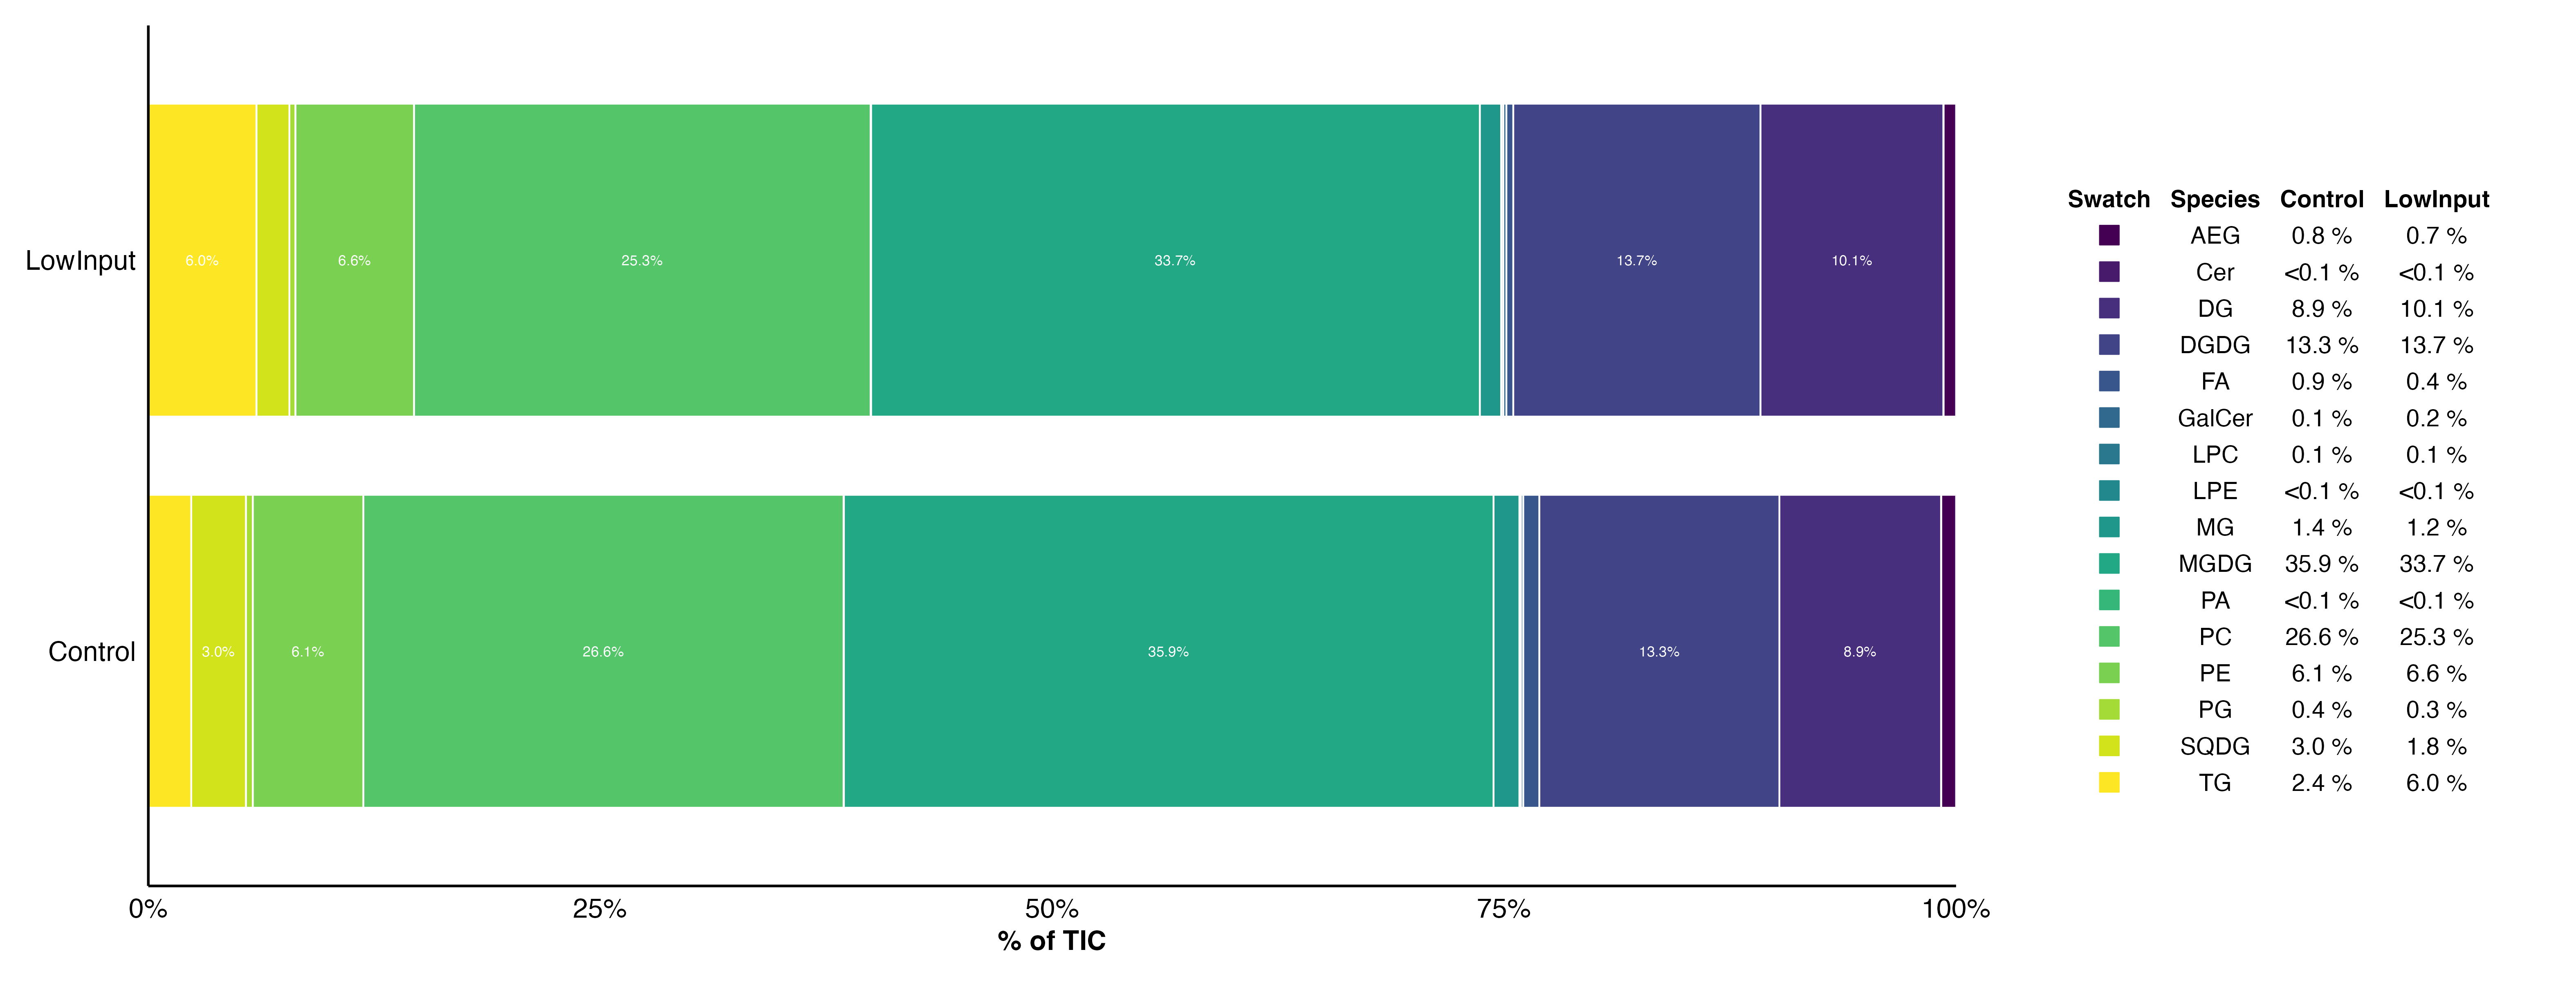
\includegraphics[width=\textwidth]{fig/main/Fig1a_lipid_species.png}
    \caption{Species‐level lipid composition (\% of TIC).}
    \label{fig:1A_lipid_species}
  \end{subfigure}

  \vspace{1em} % small vertical gap between panels

  %----------------------------------------------------
  %  (B) Bottom panel: class‐level lipid composition
  %----------------------------------------------------
  \begin{subfigure}[t]{\textwidth}
    \centering
    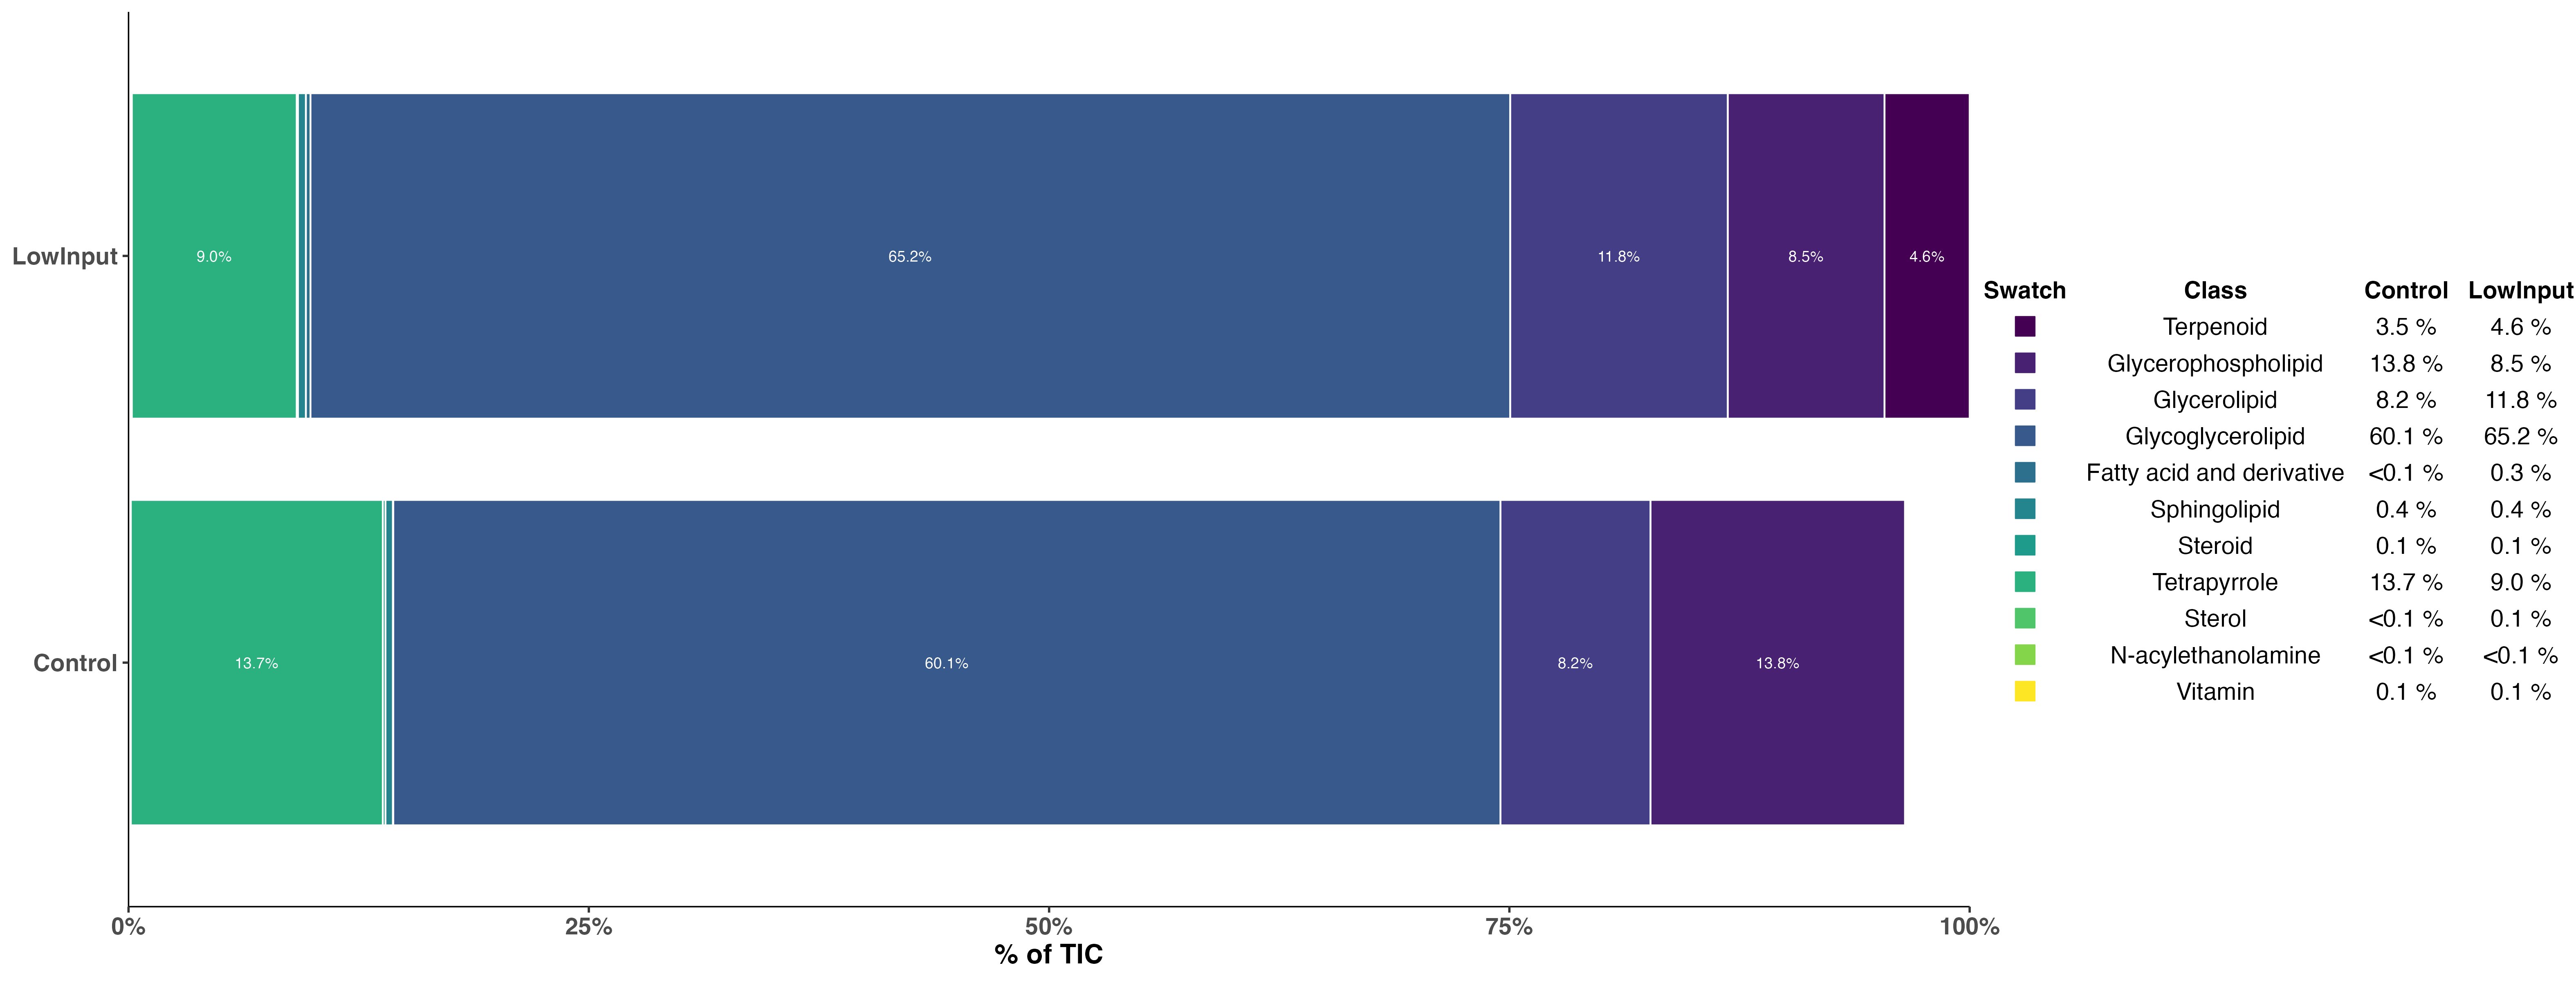
\includegraphics[width=\textwidth]{fig/main/Fig1b_lipid_class.png}
    \caption{Class‐level lipid composition (\% of TIC).}
    \label{fig:1B_lipid_class}
  \end{subfigure}

  \vspace{0.5em}

  \caption{%
    (A) Percent‐of‐TIC breakdown for individual lipid \emph{species}, averaged across all C (n = 384) and LI (n = 362) samples. Only species whose mean contribution ≥ 3 \% are labeled in‐bar.  
    (B) Percent‐of‐TIC breakdown for broader lipid \emph{classes} averaged across the same sets of samples.  
    In both panels, “Control” is shown in purple and “Low Input” in yellow.}
  \label{fig:lipid_main}
\end{figure}






\subsection*{Effect of Lowinput multistress on lipids}

\subsubsection*{Galactolipid response under the combined stress}

Contrary to the classical pattern of starvation with P, N and cold treatment, combined treatment with LI suppresses and does not improve the abundance of galactolipids (Fig.~\ref{fig:2a_ratio_lowP}):

\begin{itemize}
  \item \textbf{DGDG/PC} decreases slightly ($p<0.05$) and
        \textbf{DGDG/PE} is unchanged, indicating that digalactosyldiacylglycerol (DGDG) contracts in step with, or marginally faster than, the main phospholipids.
  \item \textbf{MGDG/PC} and \textbf{MGDG/PE} drop sharply
        ($p<0.001$), showing that
        monogalactosyldiacylglycerol (MGDG) is the class most severely depleted.
  \item The composite \textbf{ non-P_P\textsubscript{total}} metric
        \(\bigl[(\mathrm{MGDG}+\mathrm{DGDG})-(\mathrm{PC}+\mathrm{PE})\bigr]\)
        shifts downward ($p<0.001$), confirming that the global
balance of non-P: P declines rather than increases.
\end{itemize}

\paragraph{Possible Mechanism}
\begin{enumerate}
  \item \textit{Nitrogen limitation overrides the P-saving pathway.}  
        Low-N restricts UDP-galactose synthesis and translation of
        galactolipid-synthase proteins, throttling de-novo production of both
        MGDG and DGDG.
  \item \textit{Cold stress accentuates MGDG loss.}  
        Cold down-regulates MGD1/2 activity and promotes conversion of MGDG to
        DGDG or TAG, while DGDG—needed for bilayer rigidity—is merely
        stabilised, not increased.
  \item \textit{Carbon is re-routed to storage lipids.}  
        DAG released from shrinking phospholipid pools is preferentially
        channelled into TAG when nitrogen is scarce.
\end{enumerate}

Consequently, both galactolipids and phospholipids decline, with the steeper
drop in MGDG driving an overall decrease in the non-P : P ratio.
The canonical “galactolipid replacement” response is therefore only
\emph{partial and asymmetric} in sorghum when phosphorus, nitrogen and
temperature stresses co-occur: DGDG is modestly preserved for membrane
integrity, whereas MGDG and the major phospholipids are jointly curtailed.

% ------------------------------------------------------------------
%  Galactolipid behaviour (DGDG and MGDG)
% ------------------------------------------------------------------
% Place tables after the first paragraph in which they are cited.
\begin{table}[!ht]
  \begin{adjustwidth}{-2.25in}{0in} % Remove or comment out if table already fits the column
    \centering
    \caption{{\bf Canonical responses of the two major galactolipids under single stresses.}}
    \begin{tabular}{|l|c|c|p{3.8in}|}
      \hline
      \textbf{Stress} & \textbf{DGDG} & \textbf{MGDG} & \textbf{Key mechanism(s)} \\ \hline
      Low-P  & ↑ (replaces PC/PE) & ↑ (replaces PC/PE) & Diacylglycerol is redirected toward galactolipid synthesis, substituting for phospholipids under P limitation. \\ \hline
      Low-N  & ↑ / ≈ (weak retention) & ↓ & Enhanced PC breakdown releases DAG that is partly channeled to DGDG, while MGDG tends to decline as resources shift to storage lipids or other pathways. \\ \hline
      Cold   & ↑ (bilayer stabilizer) & ↓ (converted or remodeled) & Cold stress favors higher DGDG for maintaining bilayer stability; MGDG is remodeled or reduced to adjust membrane fluidity. \\ \hline
    \end{tabular}
    \begin{flushleft}
      Table notes: Arrows indicate relative changes under stress compared to control. Symbols: ↑ increase, ↓ decrease, ≈ no significant change.
    \end{flushleft}
    \label{table:galactolipid_responses}
  \end{adjustwidth}
\end{table}

\subsubsection*{Phosphatidylglycerol dynamics under multi-stress conditions}

The \texttt{PG\_retention} metric---defined as%
\[
  \log_{10}\!\Bigl(\tfrac{\text{PG}}{\sqrt{\text{PC}\cdot\text{PE}}}\Bigr)
\]
---decreases sharply under the low-input treatment
($p<0.001$;
Fig.~\ref{fig:2a_ratio_lowP}).
Thus, phosphatidylglycerol (PG) contracts \emph{faster} than the major
phospholipids PC and PE when phosphorus, nitrogen and temperature
stresses act simultaneously.
This behaviour contrasts with the classical single-stress response in
which Low-P or cold alone promotes PG retention to stabilise photosystem II
(PSII) membranes.

\paragraph{Metabolic interpretation.}
\begin{enumerate}
  \item \textbf{Nitrogen scarcity dominates PG regulation.}  
        PG biosynthesis relies on the CDP-DAG pathway, which requires
        nitrogen-rich precursors (CTP, glutamine).  Under Low-N these
        substrates---and the PG-phosphate synthase protein itself---become
        limiting, curtailing PG renewal despite any Low-P or cold demand.
  \item \textbf{Carbon diversion under cold exacerbates loss.}  
      Cold stress reallocates carbon toward soluble-sugar cryoprotectants
      and triacylglycerol (TAG) storage.  The highly unsaturated
      acyl chains that characterise thylakoid PG in grasses
      (e.g.\ 16:0/18:3 or 34:1 species in sorghum) are costly to
      assemble under carbon-limited conditions, so PG synthesis is
      curtailed in favour of stress-protective metabolites.
  \item \textbf{Photosynthetic downsizing reduces PG demand.}  
        Maintenance of PG-stabilised PSII complexes is beneficial when
        phosphorus alone is limited, but under triple stress the plant
        prioritises survival over maximal photosynthetic output.
        Thylakoid membranes are remodelled or partially dismantled,
        further lowering the need for PG.
\end{enumerate}

Taken together, the data indicate a regulatory hierarchy \(\text{Low-N} > \text{Cold} > \text{Low-P}\) for PG turnover in sorghum leaves:
nitrogen limitation constrains PG biosynthesis,
cold shifts carbon allocation away from PG, and
phosphorus stress alone is insufficient to sustain PG levels when the
other two constraints are present.

The observed decline in PG retention under field-relevant multi-stress
reveals a strategic trade-off: sorghum sacrifices part of its
photosynthetic membrane capacity to conserve nitrogen and carbon pools
needed for broader stress resilience.




% ------------------------------------------------------------------
%  PG behaviour under single stresses (matching Galactolipid layout)
% ------------------------------------------------------------------
\begin{table}[!ht]
  \begin{adjustwidth}{-2.25in}{0in} % Remove or comment out if table already fits the column
    \centering
    \caption{{\bf Canonical phosphatidylglycerol (PG) responses under single stresses.}}
    \begin{tabular}{|l|c|p{4in}|}
      \hline
      \textbf{Stress} & \textbf{PG response} & \textbf{Underlying mechanism(s)} \\ \hline
      Low-P  & ↑ Retention (PG spared) & PG is indispensable for photosystem II and can partially substitute for other phospholipids in the thylakoid membrane, so plants preferentially preserve it when phosphate is scarce. \\ \hline
      Low-N  & ↓ Retention (PG degraded) & PG synthesis relies on nitrogen-dependent CDP-DAG and PG-phosphate synthase; nitrogen limitation restricts head-group supply and enzyme abundance, reducing PG output. \\ \hline
      Cold   & ↑ Retention (stabilises PSII) & PG’s highly unsaturated acyl chains help maintain membrane fluidity and stabilise photosystems at low temperature, leading to selective retention. \\ \hline
    \end{tabular}
    \begin{flushleft}
      Table notes: Arrows indicate relative changes under stress compared with control. Symbols: ↑ increase, ↓ decrease, ≈ no significant change.
    \end{flushleft}
    \label{table:PG_responses}
  \end{adjustwidth}
\end{table}


\subsubsection*{Lysophospholipid turnover is globally suppressed under low-P + low-N + cold}

All lysophospholipid metrics decline in the low-input treatment  
(\textit{LPC/PC}, \textit{LPE/PE}, and the composite \textit{Lyso\_activity};  
each ***$p<0.001$***; Fig.~\ref{fig:2a_ratio_lowP}).  
Whereas isolated phosphorus starvation typically increases lysophospholipids
via phospholipase-mediated Pi salvage, the triple stress produces the
opposite outcome, pointing to a stress-interaction hierarchy dominated by nitrogen
limitation.

\paragraph{Metabolic interpretation.}
\begin{enumerate}
  \item \textbf{Nitrogen scarcity inhibits phospholipase turnover.}  
        PLA\textsubscript{2}/PLD\textsubscript{ζ} enzymes are N-rich; low-N
        down-regulates their transcription and limits ATP supply for their activity,
        curtailing production of LPC and LPE.
  \item \textbf{Carbon conservation discourages the lyso cycle.}  
        Re-acylation of LPC/LPE demands acyl-CoA and glycerol-3-phosphate,
        resources redirected toward TAG synthesis and soluble sugar
        cryoprotectants under cold stress.  Suppressing lyso formation avoids that
        energetic burden.
  \item \textbf{Membrane protection outweighs Pi recycling.}  
        Lysophospholipids destabilise bilayers; preventing their accumulation
        reduces cold-induced leakiness and free-fatty-acid toxicity.
\end{enumerate}

Collectively, the data indicate that maintenance of membrane integrity under
nitrogen and temperature stress overrides the classical P-scavenging
phospholipase response, even at the cost of reduced long-term phosphorus
recycling.

% ------------------------------------------------------------------
%  Lysophospholipid behaviour under single stresses
% ------------------------------------------------------------------
\begin{table}[!ht]
  \begin{adjustwidth}{-2.25in}{0in} % Remove/comment if table already fits
    \centering
    \caption{{\bf Canonical lysophospholipid responses under single stresses.}}
    \begin{tabular}{|l|c|c|p{4.0in}|}
      \hline
      \textbf{Stress} & \textbf{LPC/PC} & \textbf{LPE/PE} & \textbf{Key mechanism(s)} \\ \hline
      Low-P  & ↑ (transient) & ↑ (transient) &
      Phospholipase activation liberates Pi from PC/PE; LPC/LPE accumulate
      before being recycled. \\ \hline
      Low-N  & ↓ & ↓ &
      Plants conserve structural PC/PE; phospholipase expression and ATP supply
      decline, lowering lysophospholipid formation. \\ \hline
      Cold   & ↑ or ≈ & ↑ or ≈ &
      Membrane damage can trigger PLA-mediated hydrolysis; magnitude depends on
      genotype and acclimation. \\ \hline
    \end{tabular}
    \begin{flushleft}
      Table notes: Arrows denote typical direction of change relative to control.
      Symbols—↑ increase, ↓ decrease, ≈ no consistent change.
    \end{flushleft}
    \label{table:lyso_responses}
  \end{adjustwidth}
\end{table}



% ==========================================================
%  Neutral-lipid re-allocation under low-P + low-N + cold
% ==========================================================

\subsubsection*{Nitrogen-dominated diversion of membrane carbon into triacylglycerol storage}

All neutral-to-phospholipid ratios shift in the same direction
(Fig.~\ref{fig:2b_ratio_lowN}):

\begin{itemize}
  \item \textbf{TG/PC} rises by \(+0.50\) log\(_{10}\) units
        (≈3.2-fold; ***$p<0.001$***),
        revealing massive diversion of carbon from structural PC into
        storage TAG.
  \item \textbf{DG/PC} and \textbf{DG/Phospho} fall (both ***),
        indicating that the diacylglycerol (DG) pool is not replenished by
        new PC synthesis and is rapidly depleted.
  \item \textbf{TG/DG} increases 4.1-fold (***),
        confirming rapid DG→TAG conversion via DGAT/PDAT.
  \item \textbf{TG/Phospho} also increases sharply (***),
        underscoring the global carbon flux toward neutral lipid storage.
\end{itemize}

\paragraph{Metabolic interpretation.}
\begin{enumerate}
  \item \textbf{Low-N drives the “membrane-to-oil” shift.}\;
        Nitrogen scarcity blocks protein and phospholipid biosynthesis,
        leaving excess fixed carbon without a nitrogen sink.
        DGAT1 and PDAT1 expression is up-regulated, funnelling DG to TAG
        droplets; PDAT steals acyl chains directly from PC, deepening the
        TG/PC gap.
  \item \textbf{Cold stress amplifies TAG demand.}\;
        TAG droplets buffer free-fatty-acid toxicity and serve as an
        energy reserve for β-oxidation during low-temperature growth
        arrest, reinforcing the carbon pull toward storage.
  \item \textbf{Low-P is relegated.}\;
        In isolation, P-stress usually sends DG toward
        galactolipid synthesis; here that pathway is throttled by
        nitrogen shortage (UDP-Gal limitation), so DG is siphoned to TAG
        instead.  Hence the canonical non-P lipid replacement is muted,
        but TAG accumulation is accentuated.
\end{enumerate}

\paragraph{Physiological trade-off.}
The coordinated decrease in DG pools and surge in TAG indicates that
sorghum under field-relevant multi-stress prioritises long-term survival
(energy storage, membrane protection) over membrane turnover and rapid
growth.
This nitrogen-dominated hierarchy (Low-N \(\!>\) Cold \(\!>\) Low-P) mirrors
the lysophospholipid and PG trends described above, highlighting a
concerted re-wiring of lipid metabolism when multiple abiotic stresses
co-occur.

% ------------------------------------------------------------------
%  Canonical neutral-lipid responses under single stresses
% ------------------------------------------------------------------
\begin{table}[!ht]
  \begin{adjustwidth}{-2.25in}{0in} % remove/comment if table fits
    \centering
    \caption{{\bf Neutral-lipid (DG, TAG) behaviour under single stresses.}}
    \begin{tabular}{|l|c|c|p{4in}|}
      \hline
      \textbf{Stress} & \textbf{DG/PC} & \textbf{TG/PC} &
      \textbf{Dominant mechanism(s)} \\ \hline
      Low-P  & ↑ (DG from PL hydrolysis) & ↔ to ↑ &
      DG and Pi released by PLD/PLC; some DG diverted to galactolipids,
      modest TAG rise. \\ \hline
      Low-N  & ↓ (DG quickly consumed) & ↑↑ (strong rise) &
      DGAT/PDAT channel DG to TAG while PC synthesis slows. \\ \hline
      Cold   & ↔ or ↑ & ↑ &
      TAG buffers unsaturated FA surplus and stores excess carbon
      during growth arrest. \\ \hline
    \end{tabular}
    \begin{flushleft}
      Table notes: arrows indicate typical change vs.\ control
      (↑ increase, ↓ decrease, ↔ little change).  The triple-stress
      response matches the Low-N column, confirming nitrogen dominance.
    \end{flushleft}
    \label{table:neutral_stress_single}
  \end{adjustwidth}
\end{table}



% ------------------------------------------------------------------
%  Classic neutral-lipid responses under single stresses
% ------------------------------------------------------------------
\begin{table}[!ht]
  \begin{adjustwidth}{-2.25in}{0in} % remove if table fits page
    \centering
    \caption{{\bf Canonical neutral-lipid (DG and TAG) responses under single stresses.}}
    \begin{tabular}{|l|c|c|p{4in}|}
      \hline
      \textbf{Stress} & \textbf{DG/PC} & \textbf{TG/PC} & \textbf{Key mechanism(s)} \\ \hline
      Low-P  & ↑ (DG from PC hydrolysis) & ↔ or ↑ (TAG may rise slightly) &
      Phospholipase C/PLD liberate DG and Pi; some DG converted to DGDG, some to TAG. \\ \hline
      Low-N  & ↓ (DG rapidly consumed) & ↑↑ (strong TAG accumulation) &
      DAG is channelled to TAG as protein synthesis slows, storing excess carbon. \\ \hline
      Cold   & ↔ or ↑ (membrane remodelling) & ↑ (carbon sink during growth arrest) &
      Acyl-editing and DGAT activity increase; TAG buffers FA imbalance under chill. \\ \hline
    \end{tabular}
    \begin{flushleft}
      Table notes: Arrows show typical direction of change relative to control.
      Symbols—↑ increase, ↓ decrease, ↔ little or no change.
    \end{flushleft}
    \label{table:neutral_lipid_responses}
  \end{adjustwidth}
\end{table}


% ==========================================================
%  Cold-dominated reshaping of the chloroplast glycolipid triad
% ==========================================================

\subsubsection*{Cold stress overrides nutrient limitations to prioritise DGDG and suppress SQDG}

Even in the presence of nitrogen and phosphorus shortages, cold imposes a
distinct thylakoid lipid signature (Fig.~\ref{fig:2c_ratio_cold}):

\begin{itemize}
  \item \textbf{MGDG/DGDG} decreases by $-0.28$ log$_{10}$ units
        (***$p<0.001$***), reflecting preferential enrichment of
        digalactosyldiacylglycerol (DGDG) over monogalactosyldiacylglycerol (MGDG).
  \item \textbf{SQDG/DGDG} and \textbf{SQDG/MGDG} decline even more steeply
        (both ***), while \textbf{SQDG/total} also drops (***),
        indicating a concerted collapse of the sulfolipid pool.
  \item Despite the lower MGDG/DGDG ratio, both \textbf{DGDG/total} and
        \textbf{MGDG/total} rise (***), showing that total galactolipid
        content still increases at the expense of phospholipids; DGDG simply
        rises faster than MGDG.
\end{itemize}

\paragraph{Hierarchy of stress priorities: \textit{Cold > Low-P > Low-N}.}
\begin{enumerate}
  \item \textbf{DGDG is non-negotiable for PSII stability at low temperature.}  
        Cold induces MGDG\,$\rightarrow$\,DGDG conversion to minimise
        negative-curvature lipids and prevent hexagonal\,II phase formation.
        The strong DGDG enrichment persists even when N and P are scarce.
  \item \textbf{MGDG increases in absolute terms but lags behind DGDG.}  
        Cold still drives some de-novo MGDG synthesis; however,
        the faster rise of DGDG tips the MGDG/DGDG ratio downward.
  \item \textbf{SQDG is sacrificed to conserve sulfur and carbon.}  
        Low-N constrains sulfite assimilation (glutamine/ATP limitation) and
        down-regulates SQD1/SQD2; cold diverts carbon to raffinose
        cryoprotectants.  The plant therefore de-prioritises SQDG,
        reallocating sulfur to glutathione and other defences.
\end{enumerate}

\paragraph{Physiological consequence.}
The cold-first hierarchy produces a \emph{DGDG-dominant, SQDG-poor} membrane,
ensuring thylakoid integrity while tolerating reduced phosphorus recycling
and sulfur use.  This pattern contrasts with single-stress responses
(Table~\ref{table:triad_single_stress}) and highlights that field crops in
cold climates may commit metabolic resources to DGDG maintenance before
addressing P or N constraints.

% ------------------------------------------------------------------
%  Canonical chloroplast glycolipid responses under single stresses
%  (unchanged but repeated for context)
% ------------------------------------------------------------------
\begin{table}[!ht]
  \begin{adjustwidth}{-2.25in}{0in}  % Remove/comment if table already fits
    \centering
    \caption{{\bf Typical behaviour of thylakoid glycolipids under single stresses.}}
    \begin{tabular}{|l|c|c|c|p{3.8in}|}
      \hline
      \textbf{Stress} & \textbf{DGDG} & \textbf{MGDG} & \textbf{SQDG} &
      \textbf{Key mechanism(s)} \\ \hline
      Low-P  & ↑ (replace PC/PE) & ↑ (replace PC/PE) & ↑ (replace PG) &
      Galactose pathway activated; SQDG substitutes for anionic PG. \\ \hline
      Low-N  & ↔ or ↓ & ↓ & ↓ &
      Nitrogen shortage limits galactolipid synthases and sulfur uptake. \\ \hline
      Cold   & ↑ (bilayer stabiliser) & ↓ (converted to DGDG) & ↔ or ↑ &
      Fluidity control via MGDG→DGDG conversion; SQDG depends on S status. \\ \hline
    \end{tabular}
    \begin{flushleft}
      Table notes: arrows indicate usual direction of change (↑ increase, ↓ decrease, ↔ minimal change).  
      The triple-stress profile (↑ DGDG, modest ↑ MGDG, ↓ SQDG) matches the cold column, confirming cold dominance over nutrient stresses.
    \end{flushleft}
    \label{table:triad_single_stress}
  \end{adjustwidth}
\end{table}

\subsubsection*{Diacylglycerol as a Central Hub in Stress Lipid Remodeling}

Although our primary focus has been on the balance between membrane and storage lipids (e.g.\ PC vs.\ DGDG/MGDG under low‑P, or DG/TG under low‑N), diacylglycerol (DAG) emerges as a critical intermediate across all three stresses. DAG sits at the crossroads of membrane turnover, TAG synthesis, and signaling, so we summarize its multifaceted roles below.

\paragraph{Cold acclimation.}  
In cold‑acclimated sorghum leaves, the DAG pool (reflected in the DG\_Phospho and DG\_PC contrasts) is modestly elevated (ΔZ ≈ +1 SD, p < 0.001). This suggests enhanced phospholipid deacylation or reduced PC/PE biosynthesis—both routes liberate DAG. Functionally, increased DAG may help maintain bilayer fluidity at low temperature and feed sn‑1,2‑DAG to DGK enzymes to generate phosphatidic acid (PA), a known cold‐responsive signal.

\paragraph{Phosphorus deprivation.}  
Under P limitation, while galactolipids take center stage, DAG also shifts (DG\_Phospho ΔZ ≈ +2 SD, p < 0.001), indicating that phospholipid turnover contributes DAG backbones. These DAG molecules may be transient intermediates en route to TAG (via DGAT) or PA, or they may even form alternative non‑P glycerolipids like glucuronosyldiacylglycerol (as reported in other species).

\paragraph{Nitrogen limitation.}  
The Low‑N treatments show the largest DAG/PC and TG/DG shifts (ΔZ > +3 SD), pinpointing DAG both as the product of membrane phospholipid breakdown and the substrate for TAG accumulation. This dual role—not just as a passive by‑product but as the major conduit of carbon into lipid droplets—highlights DAG’s centrality in rerouting carbon when N for protein synthesis is scarce.

---

By weaving DAG’s behavior into each of your three main subsections (Low‑P, Low‑N, Cold), you keep your narrative tight and hierarchical, yet still give DAG the distinct attention it merits.



\subsection*{Multivariate structure of lipid profiles}

\subsection*{Genome-wide association study (GWAS) of lipids}

\subsection*{Pathway identification}



%--------------------------------------------------------------------
\bibliographystyle{plainnat}
\bibliography{lipid_refs}



\section*{Discussion}
Something something lipids are good. 


\section*{Conclusion}

because we can For more information, see \nameref{S1_Appendix}.

\section*{Supporting information}

% Include only the SI item label in the paragraph heading. Use the \nameref{label} command to cite SI items in the text.
\paragraph*{S1 Fig.}
\label{S1_Fig}
{\bf Bold the title sentence.} Add descriptive text after the title of the item (optional).

\paragraph*{S2 Fig.}
\label{S2_Fig}
{\bf Lorem ipsum.} Maecenas convallis mauris sit amet sem ultrices gravida. Etiam eget sapien nibh. Sed ac ipsum eget enim egestas ullamcorper nec euismod ligula. Curabitur fringilla pulvinar lectus consectetur pellentesque.

\paragraph*{S1 File.}
\label{S1_File}
{\bf Lorem ipsum.}  Maecenas convallis mauris sit amet sem ultrices gravida. Etiam eget sapien nibh. Sed ac ipsum eget enim egestas ullamcorper nec euismod ligula. Curabitur fringilla pulvinar lectus consectetur pellentesque.

\paragraph*{S1 Video.}
\label{S1_Video}
{\bf Lorem ipsum.}  Maecenas convallis mauris sit amet sem ultrices gravida. Etiam eget sapien nibh. Sed ac ipsum eget enim egestas ullamcorper nec euismod ligula. Curabitur fringilla pulvinar lectus consectetur pellentesque.

\paragraph*{S1 Appendix.}
\label{S1_Appendix}
{\bf Lorem ipsum.} Maecenas convallis mauris sit amet sem ultrices gravida. Etiam eget sapien nibh. Sed ac ipsum eget enim egestas ullamcorper nec euismod ligula. Curabitur fringilla pulvinar lectus consectetur pellentesque.

\paragraph*{S1 Table.}
\label{S1_Table}
{\bf Lorem ipsum.} Maecenas convallis mauris sit amet sem ultrices gravida. Etiam eget sapien nibh. Sed ac ipsum eget enim egestas ullamcorper nec euismod ligula. Curabitur fringilla pulvinar lectus consectetur pellentesque.

\section*{Acknowledgments}
Me, myself and I

\nolinenumbers

% Either type in your references using
% \begin{thebibliography}{}
% \bibitem{}
% Text
% \end{thebibliography}
%
% or
%
% Compile your BiBTeX database using our plos2015.bst
% style file and paste the contents of your .bbl file
% here. See http://journals.plos.org/plosone/s/latex for 
% step-by-step instructions.
% 
\begin{thebibliography}{10}

\bibitem{bib1}
Conant GC, Wolfe KH.
\newblock {{T}urning a hobby into a job: how duplicated genes find new
  functions}.
\newblock Nat Rev Genet. 2008 Dec;9(12):938--950.

\bibitem{bib2}
Ohno S.
\newblock Evolution by gene duplication.
\newblock London: George Alien \& Unwin Ltd. Berlin, Heidelberg and New York:
  Springer-Verlag.; 1970.

\bibitem{bib3}
Magwire MM, Bayer F, Webster CL, Cao C, Jiggins FM.
\newblock {{S}uccessive increases in the resistance of {D}rosophila to viral
  infection through a transposon insertion followed by a {D}uplication}.
\newblock PLoS Genet. 2011 Oct;7(10):e1002337.

\end{thebibliography}

%==========================================
%   Start the Supplementary Material section
%==========================================
\FloatBarrier
\section*{Supplementary Material}
\beginsupplement


%========================================================
%  Supplementary Figure S1 – TIC traces
%========================================================
\begin{figure}[htp]
  \centering

  % ---------- panel A: Control TIC ----------
  \begin{subfigure}[t]{\textwidth}
    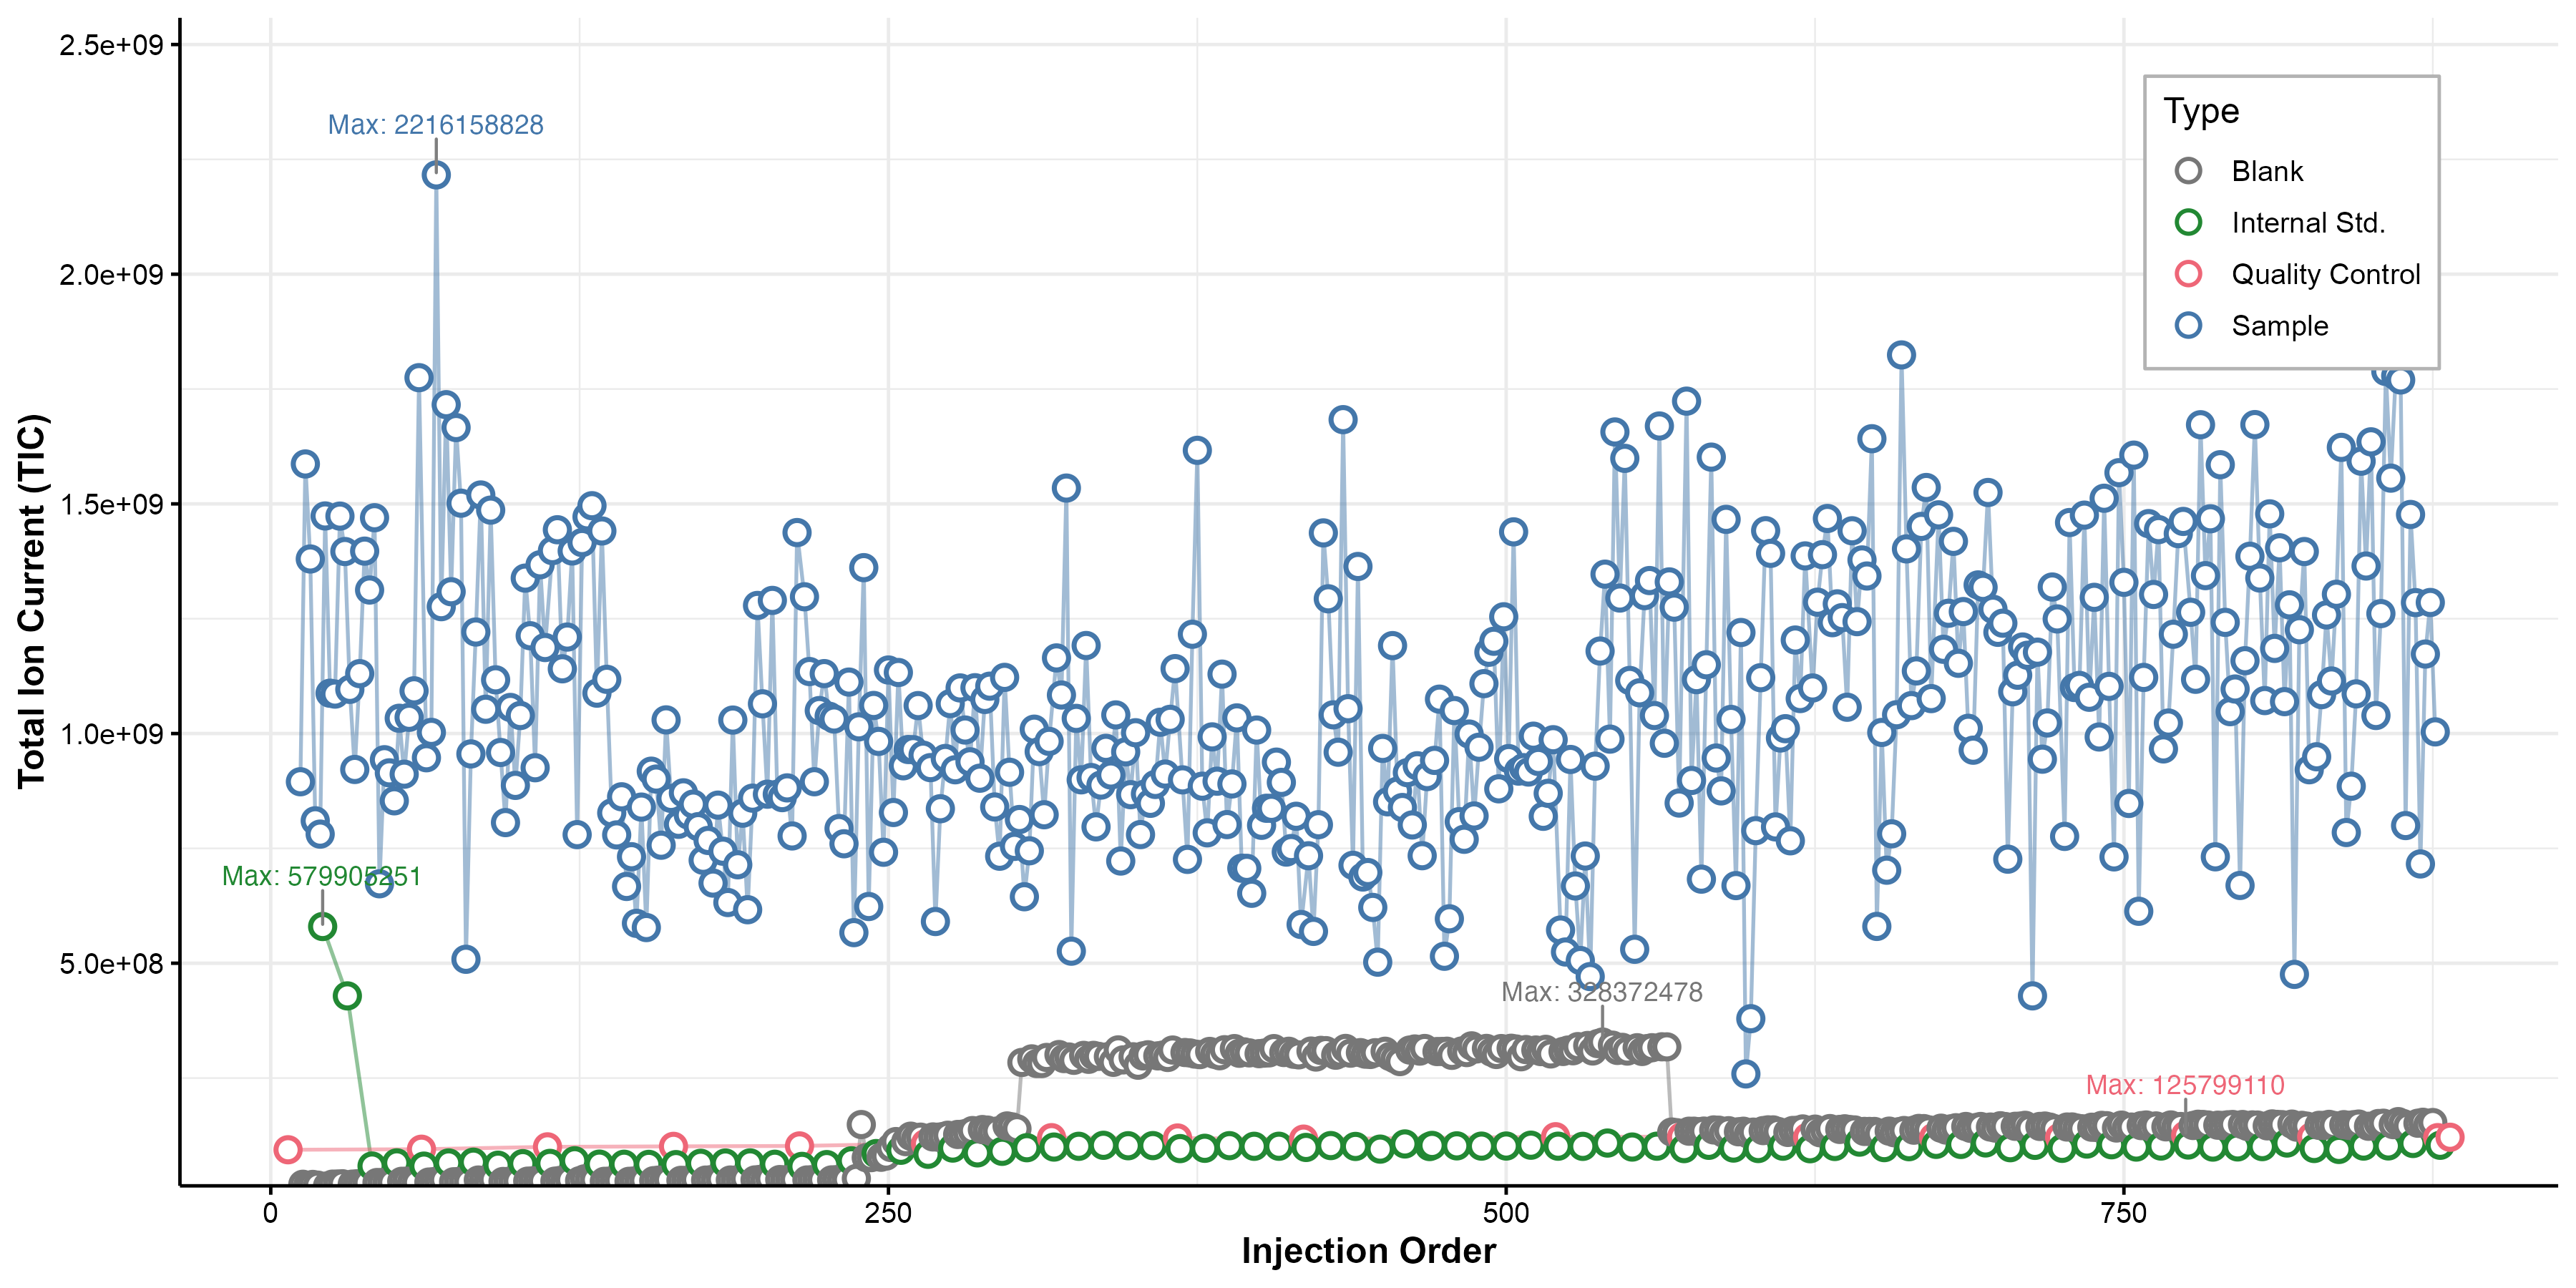
\includegraphics[width=\linewidth]{fig/supp/SuppFig_1A_TIC_Control}
    \caption{Total ion current vs.\ injection order for Control samples.}
    \label{fig:S1A}
  \end{subfigure}

  \vspace{1em}

  % ---------- panel B: Low-Input TIC ----------
  \begin{subfigure}[t]{\textwidth}
    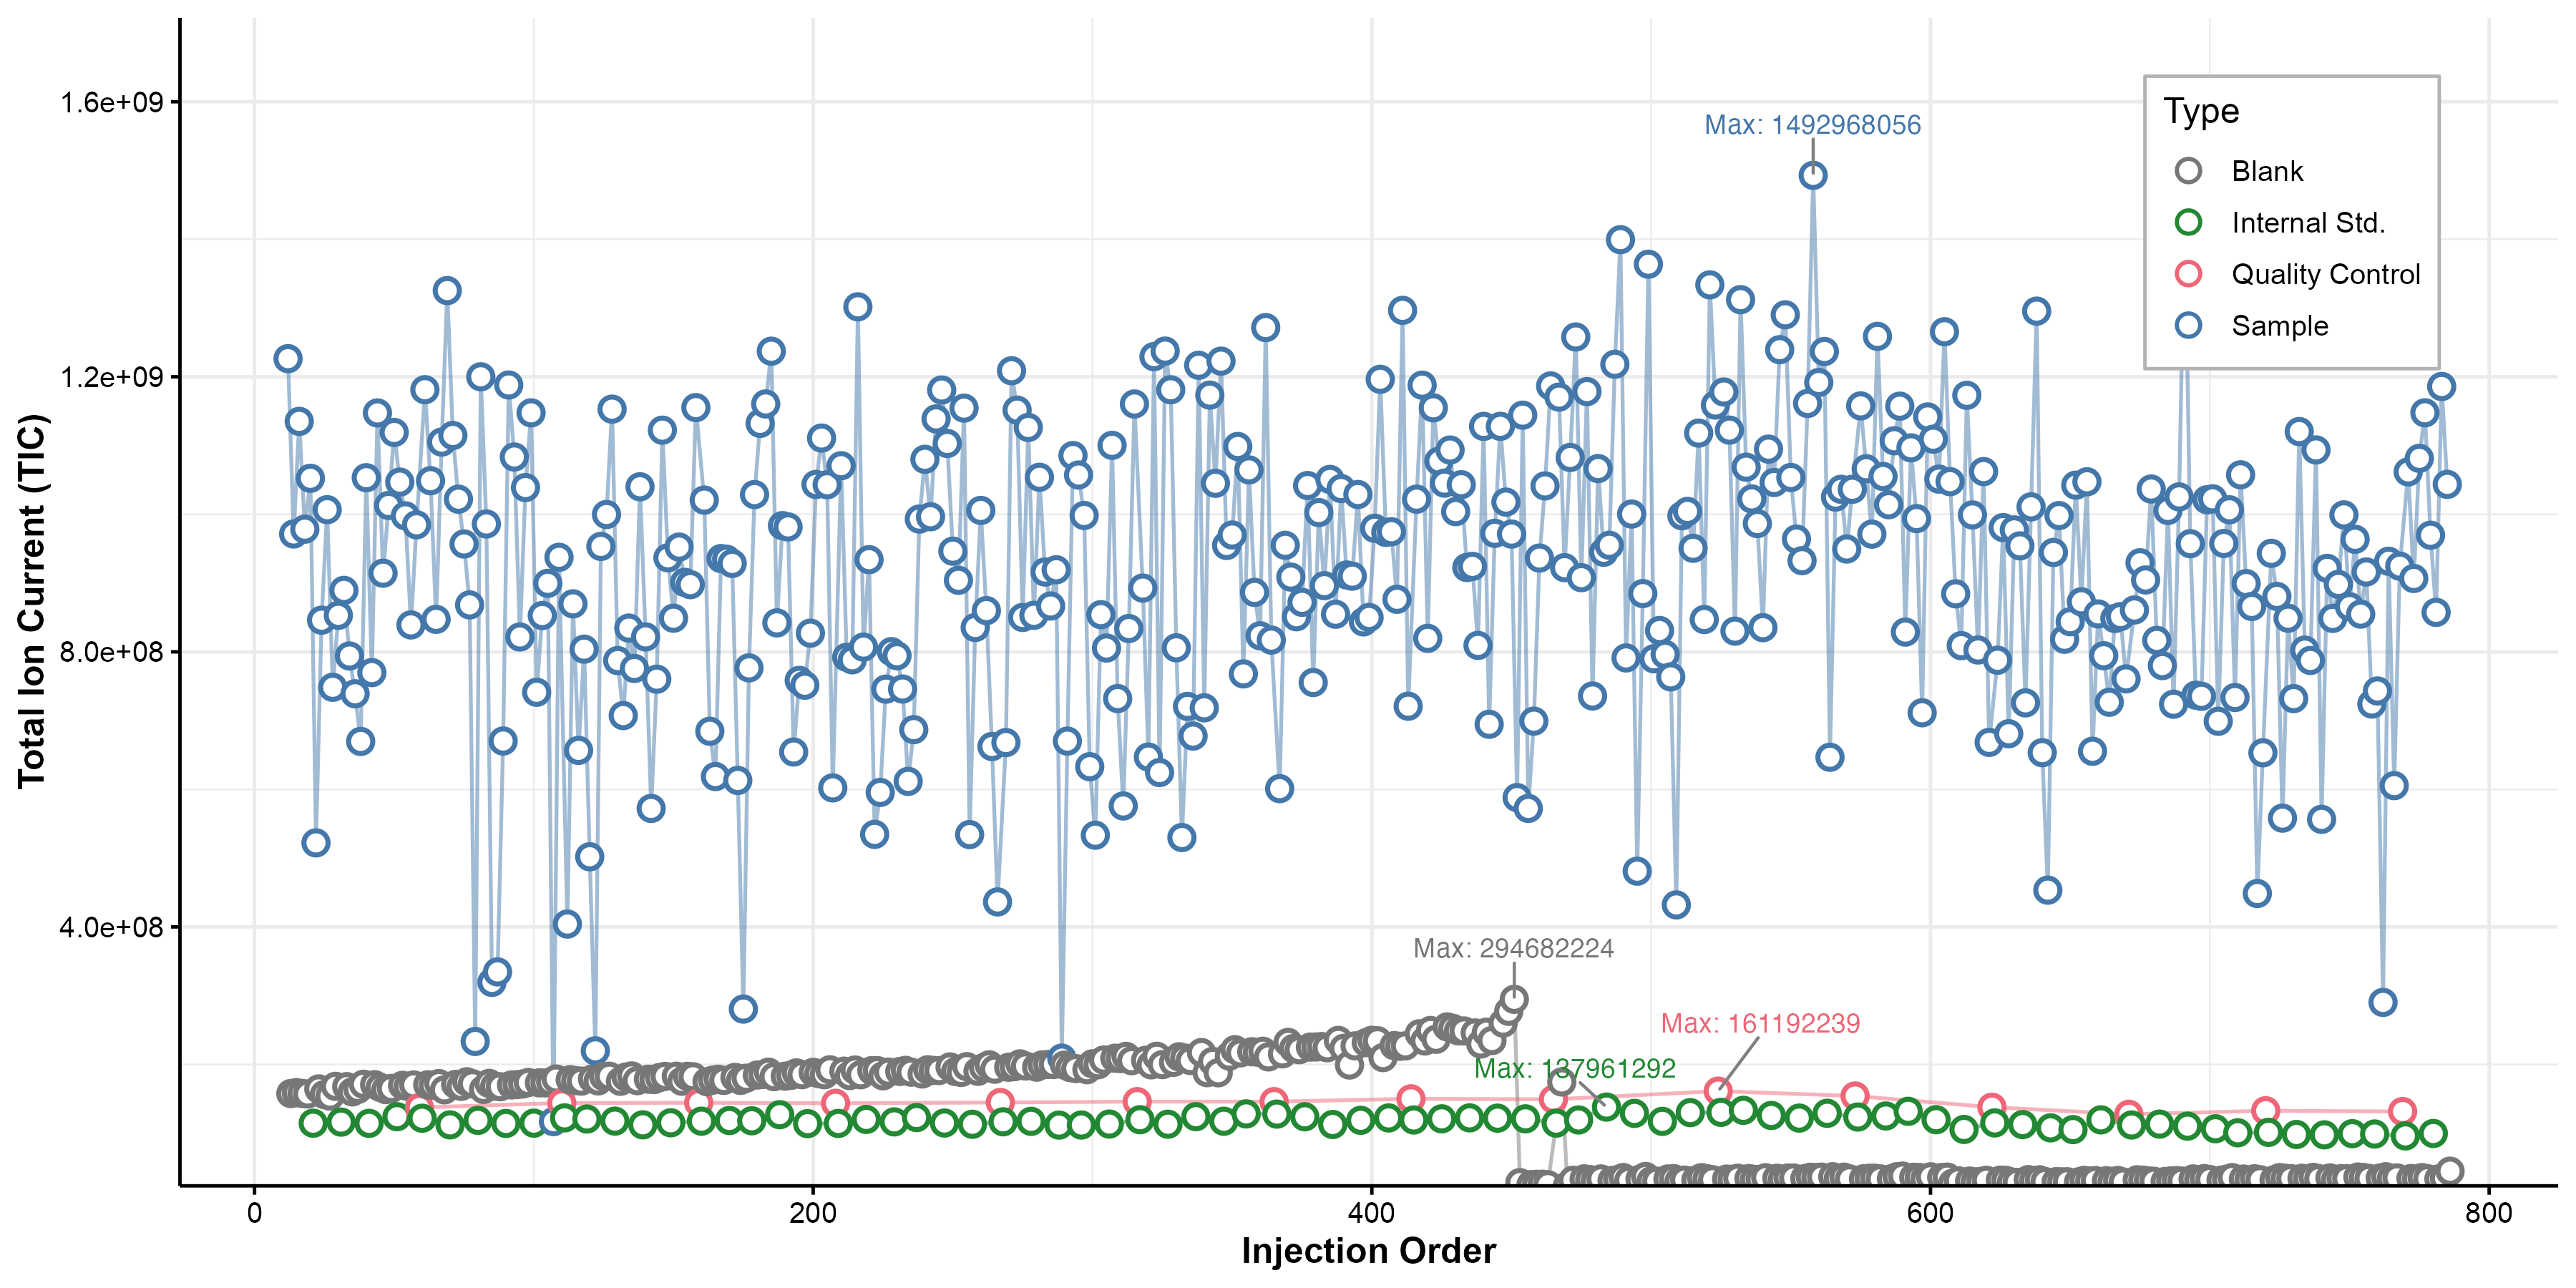
\includegraphics[width=\linewidth]{fig/supp/SuppFig_1B_TIC_LowInput.png}
    \caption{Total ion current vs.\ injection order for Low-Input samples.}
    \label{fig:S1B}
  \end{subfigure}

  \caption{TIC traces for all injections.  (A) Control, (B) Low-Input.}
  \label{fig:S1}
\end{figure}



%========================================================
%  Supplementary Figure S2 - SERFF RSD & PCA results
%========================================================
\begin{figure}[htp]
  \centering

  % ---------- row 1 ----------
  \begin{subfigure}[t]{0.48\textwidth}
    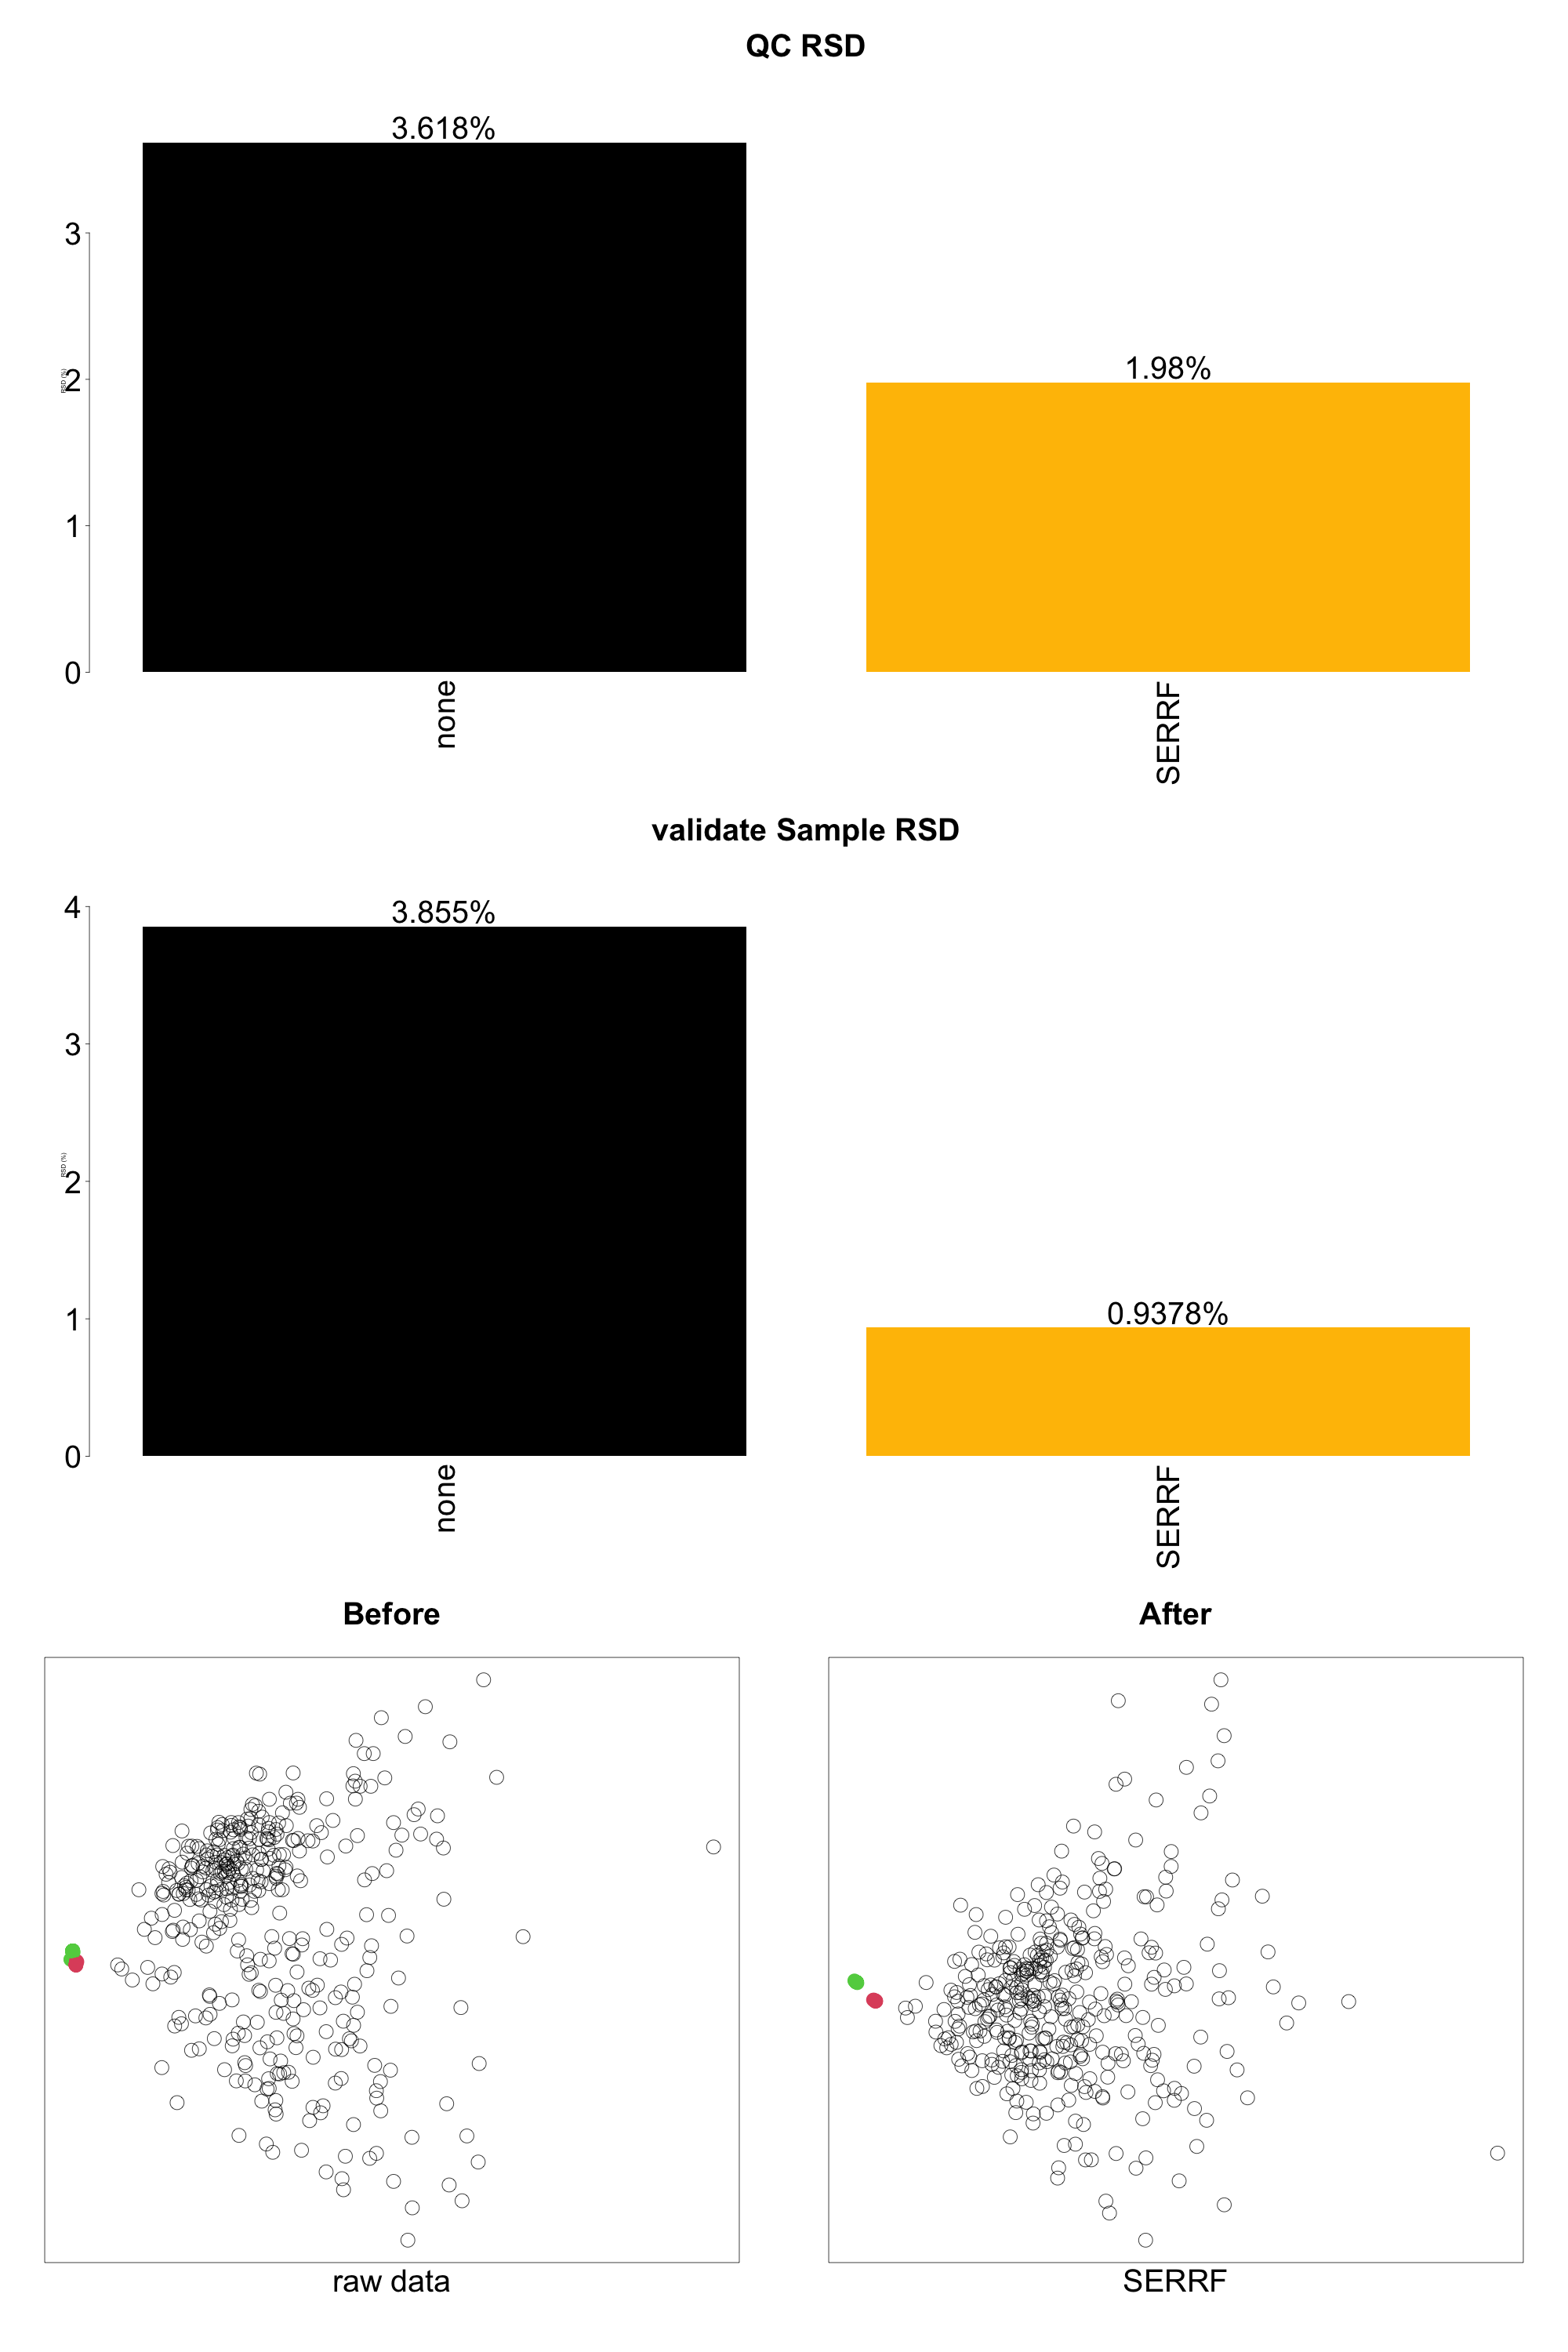
\includegraphics[width=\linewidth]{fig/supp/SuppFig_2A_RSD_PCA_Control.png}
    \caption{Control.}
    \label{fig:S2A}
  \end{subfigure}\hfill
  \begin{subfigure}[t]{0.48\textwidth}
    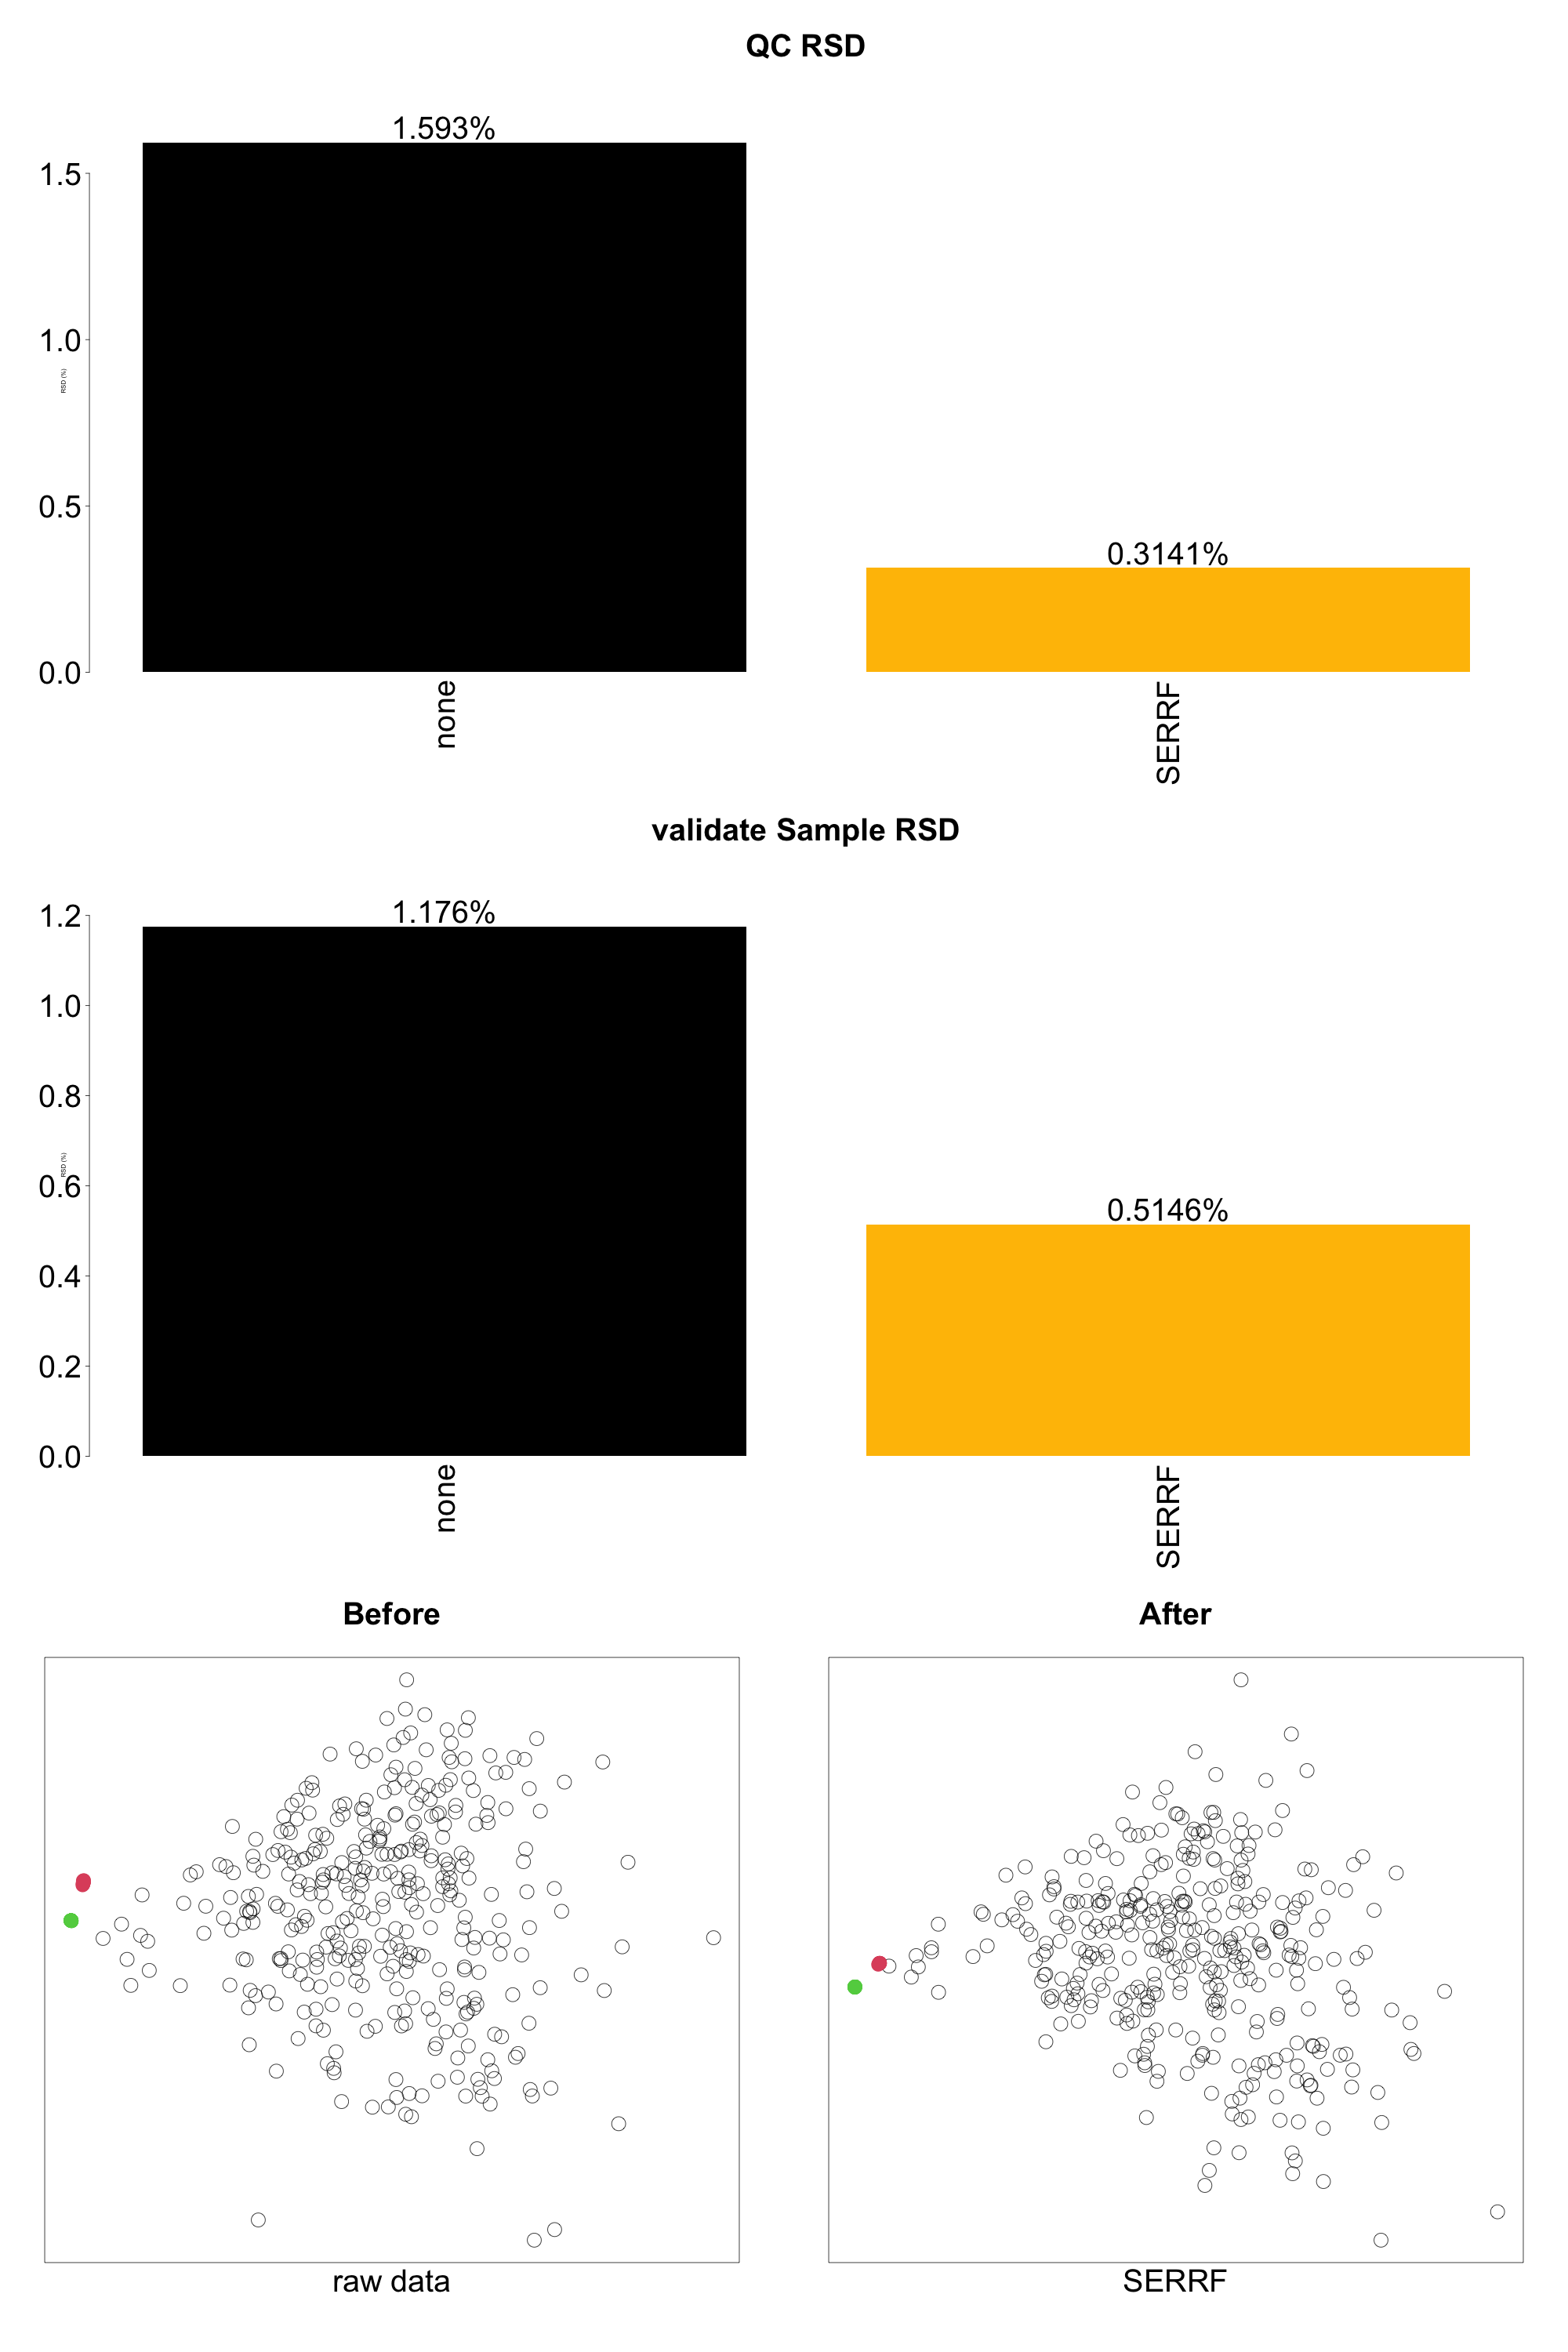
\includegraphics[width=\linewidth]{fig/supp/SuppFig_2B_RSD_PCA_Lowinput.png}
    \caption{Low‐Input.}
    \label{fig:S2B}
  \end{subfigure}

  \caption{
    SERRF-normalized quality metrics across injections.  
    (\textbf{A}) Control samples: per‐feature RSD distributions (boxplot) and PCA of QC vs.\ samples.  
    (\textbf{B}) Low‐Input samples: same metrics after SERRF correction.  
    Both panels demonstrate tight RSDs (most features<15 %) and clear separation of QC from biological samples in PC1/PC2.
  }
  \label{fig:S2}
\end{figure}







%========================================================
%  Supplementary Figure S3 - Lipid species/class count   (panels A, B, and C)
%========================================================
\begin{figure}[htp]
  \centering

  % ---------- row 1 ----------
  \begin{subfigure}[t]{0.48\textwidth}
    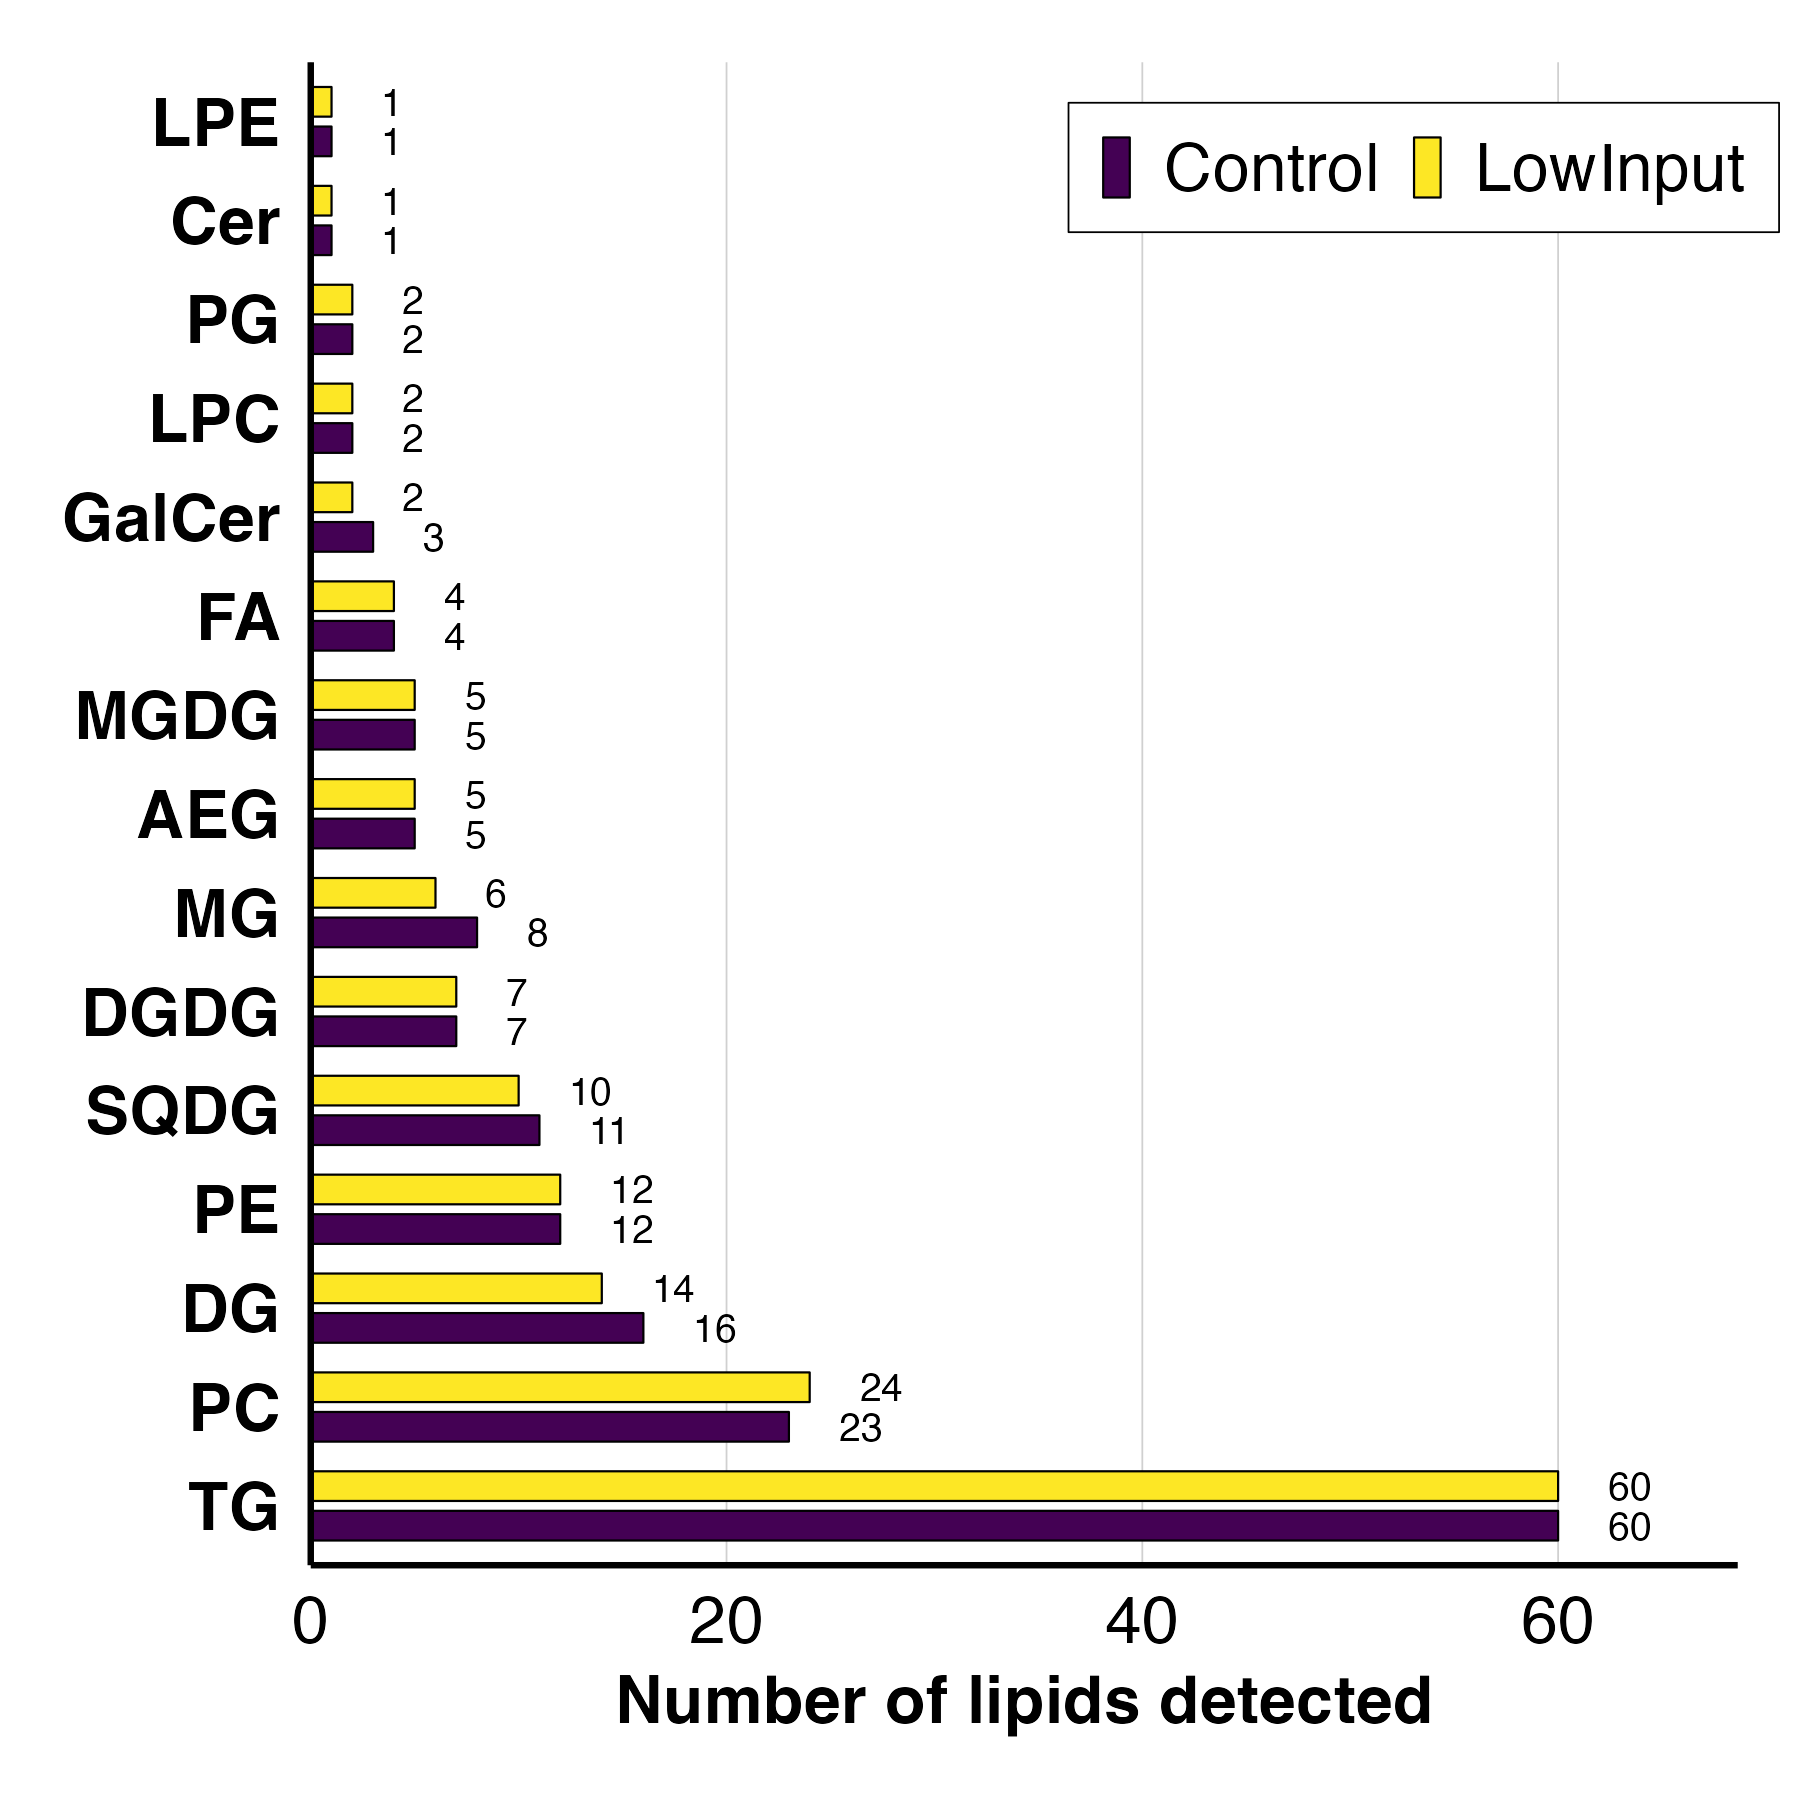
\includegraphics[width=\linewidth]{fig/supp/SuppFig_3A_Lipid_Counts}
    \caption{Number of lipid \textit{species}.}
    \label{fig:S3A}
  \end{subfigure}\hfill
  \begin{subfigure}[t]{0.48\textwidth}
    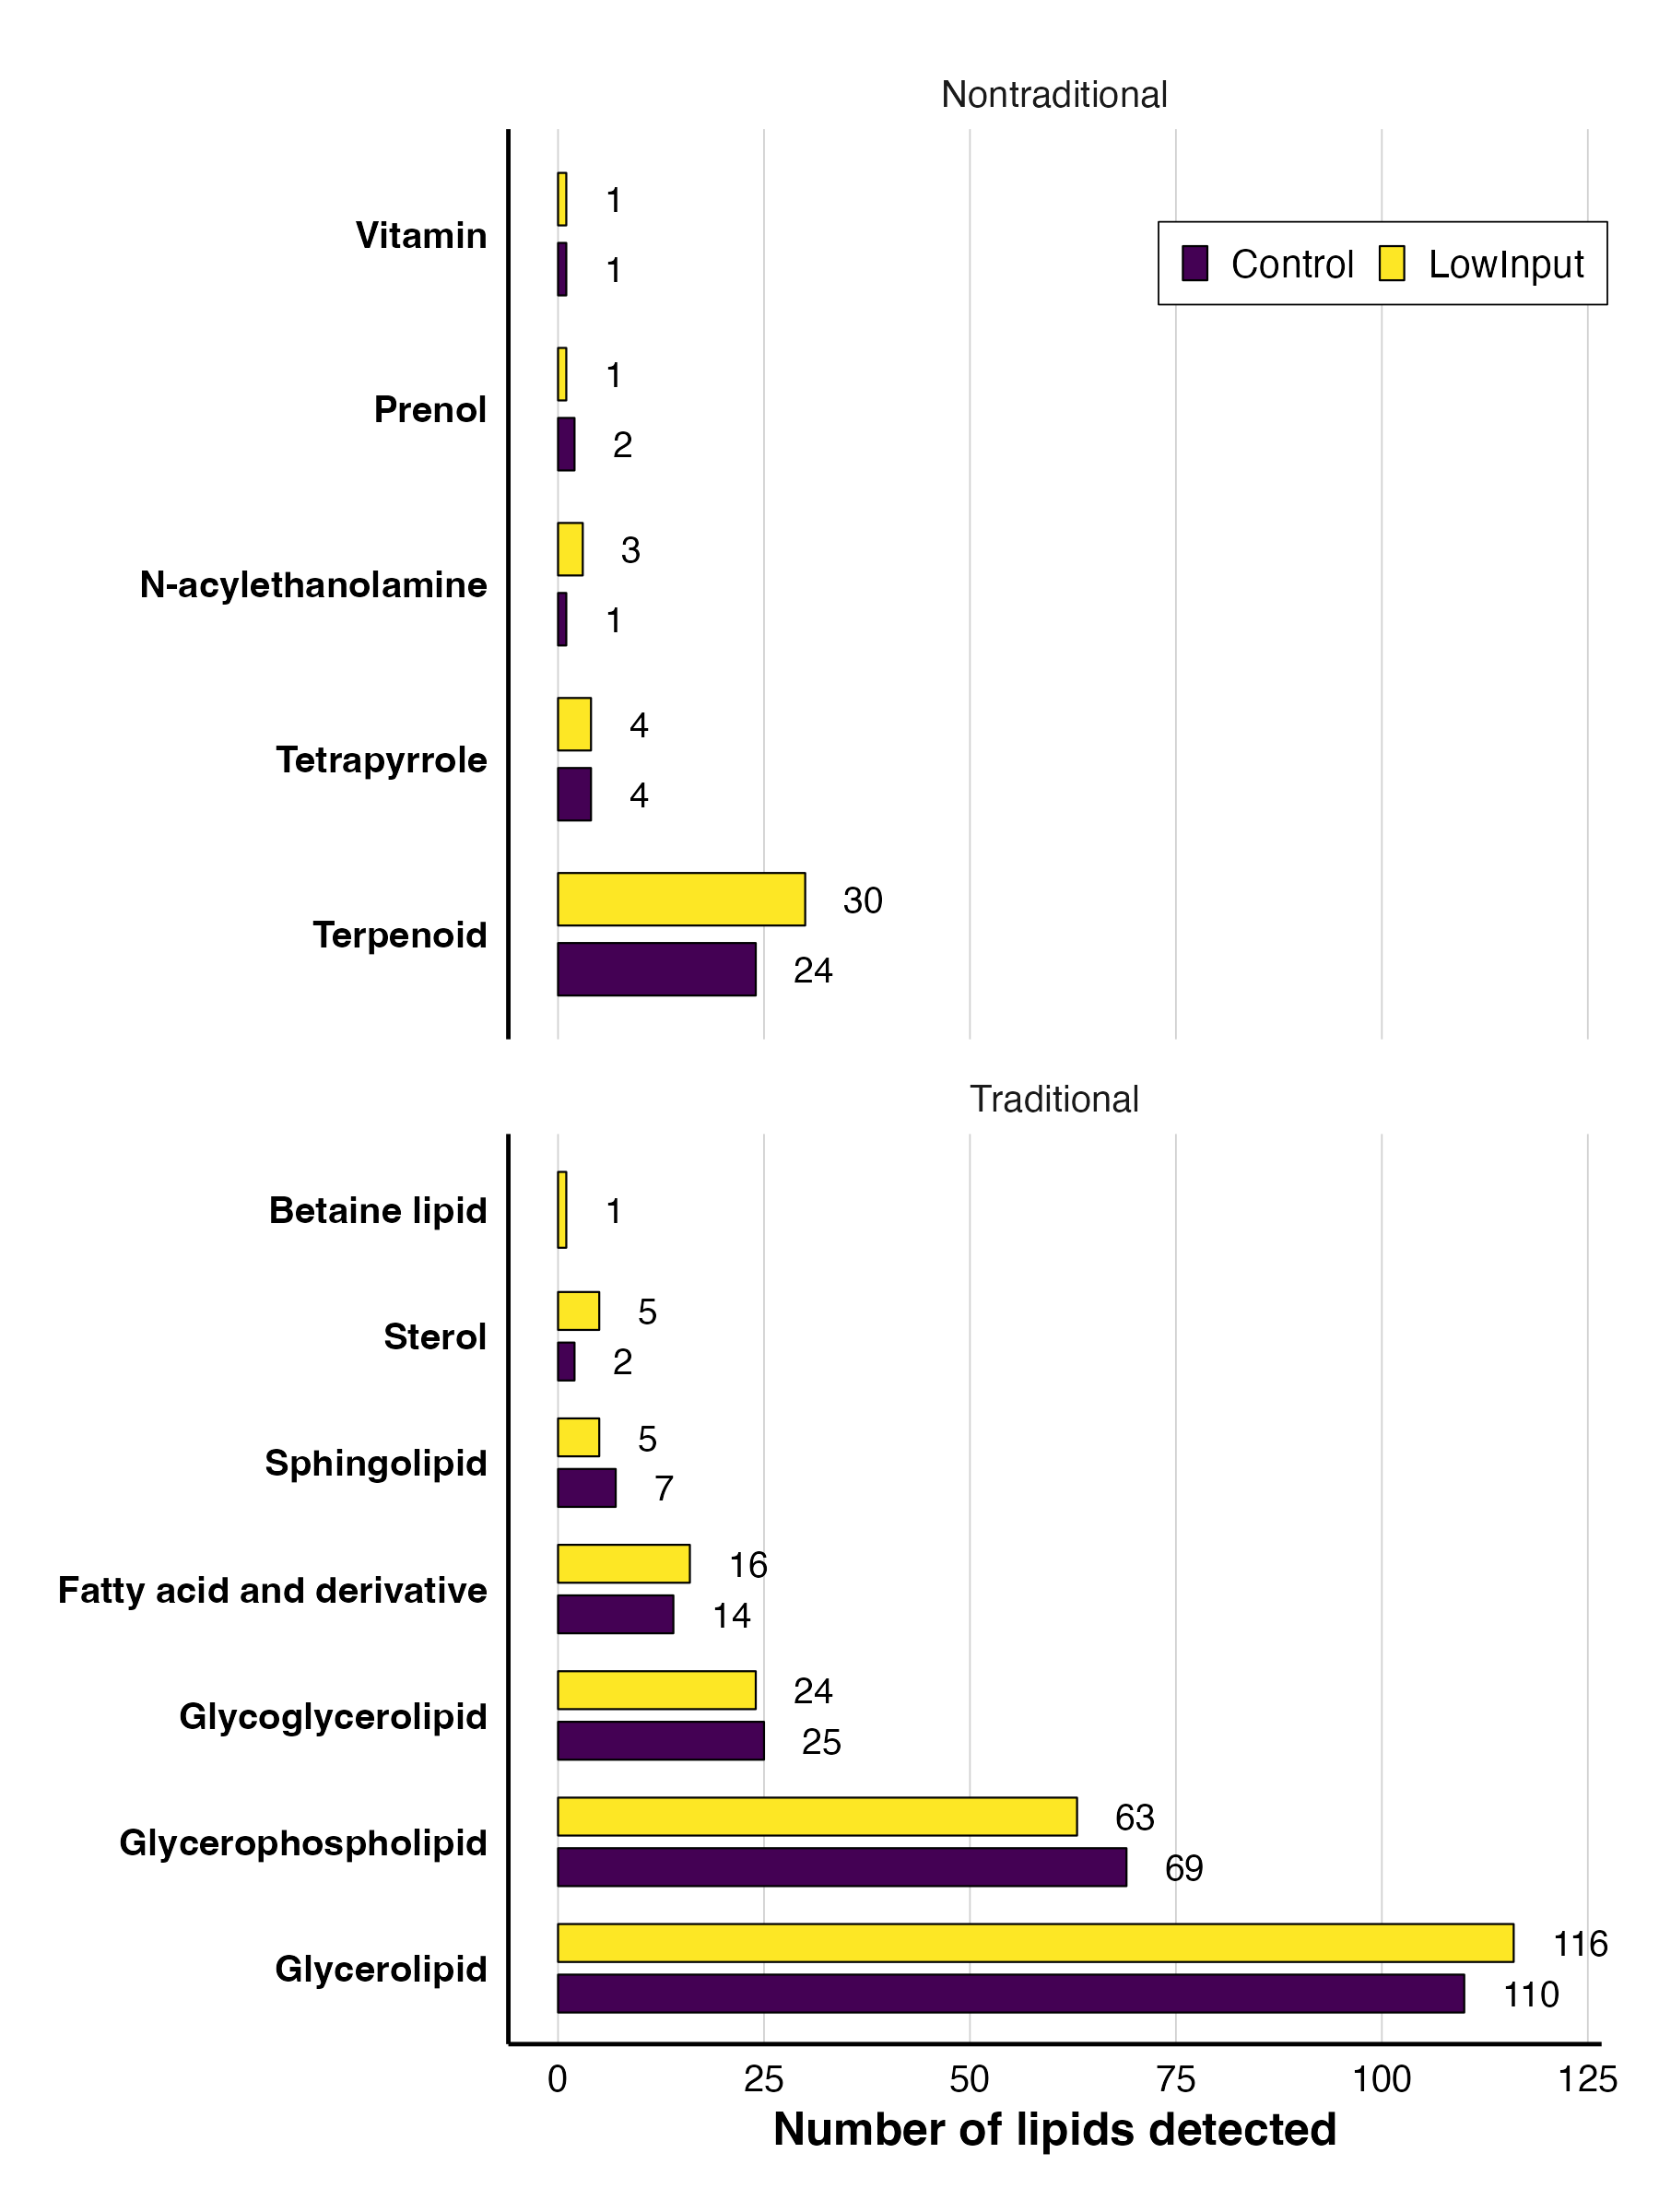
\includegraphics[width=\linewidth]{fig/supp/SuppFig_3B_Lipid_Class_Counts}
    \caption{Number of lipid \textit{classes}.}
    \label{fig:S3B}
  \end{subfigure}

  \vspace{1em}

  % ---------- row 2 (centred) ----------
  \begin{subfigure}[t]{0.55\textwidth}
    \centering
    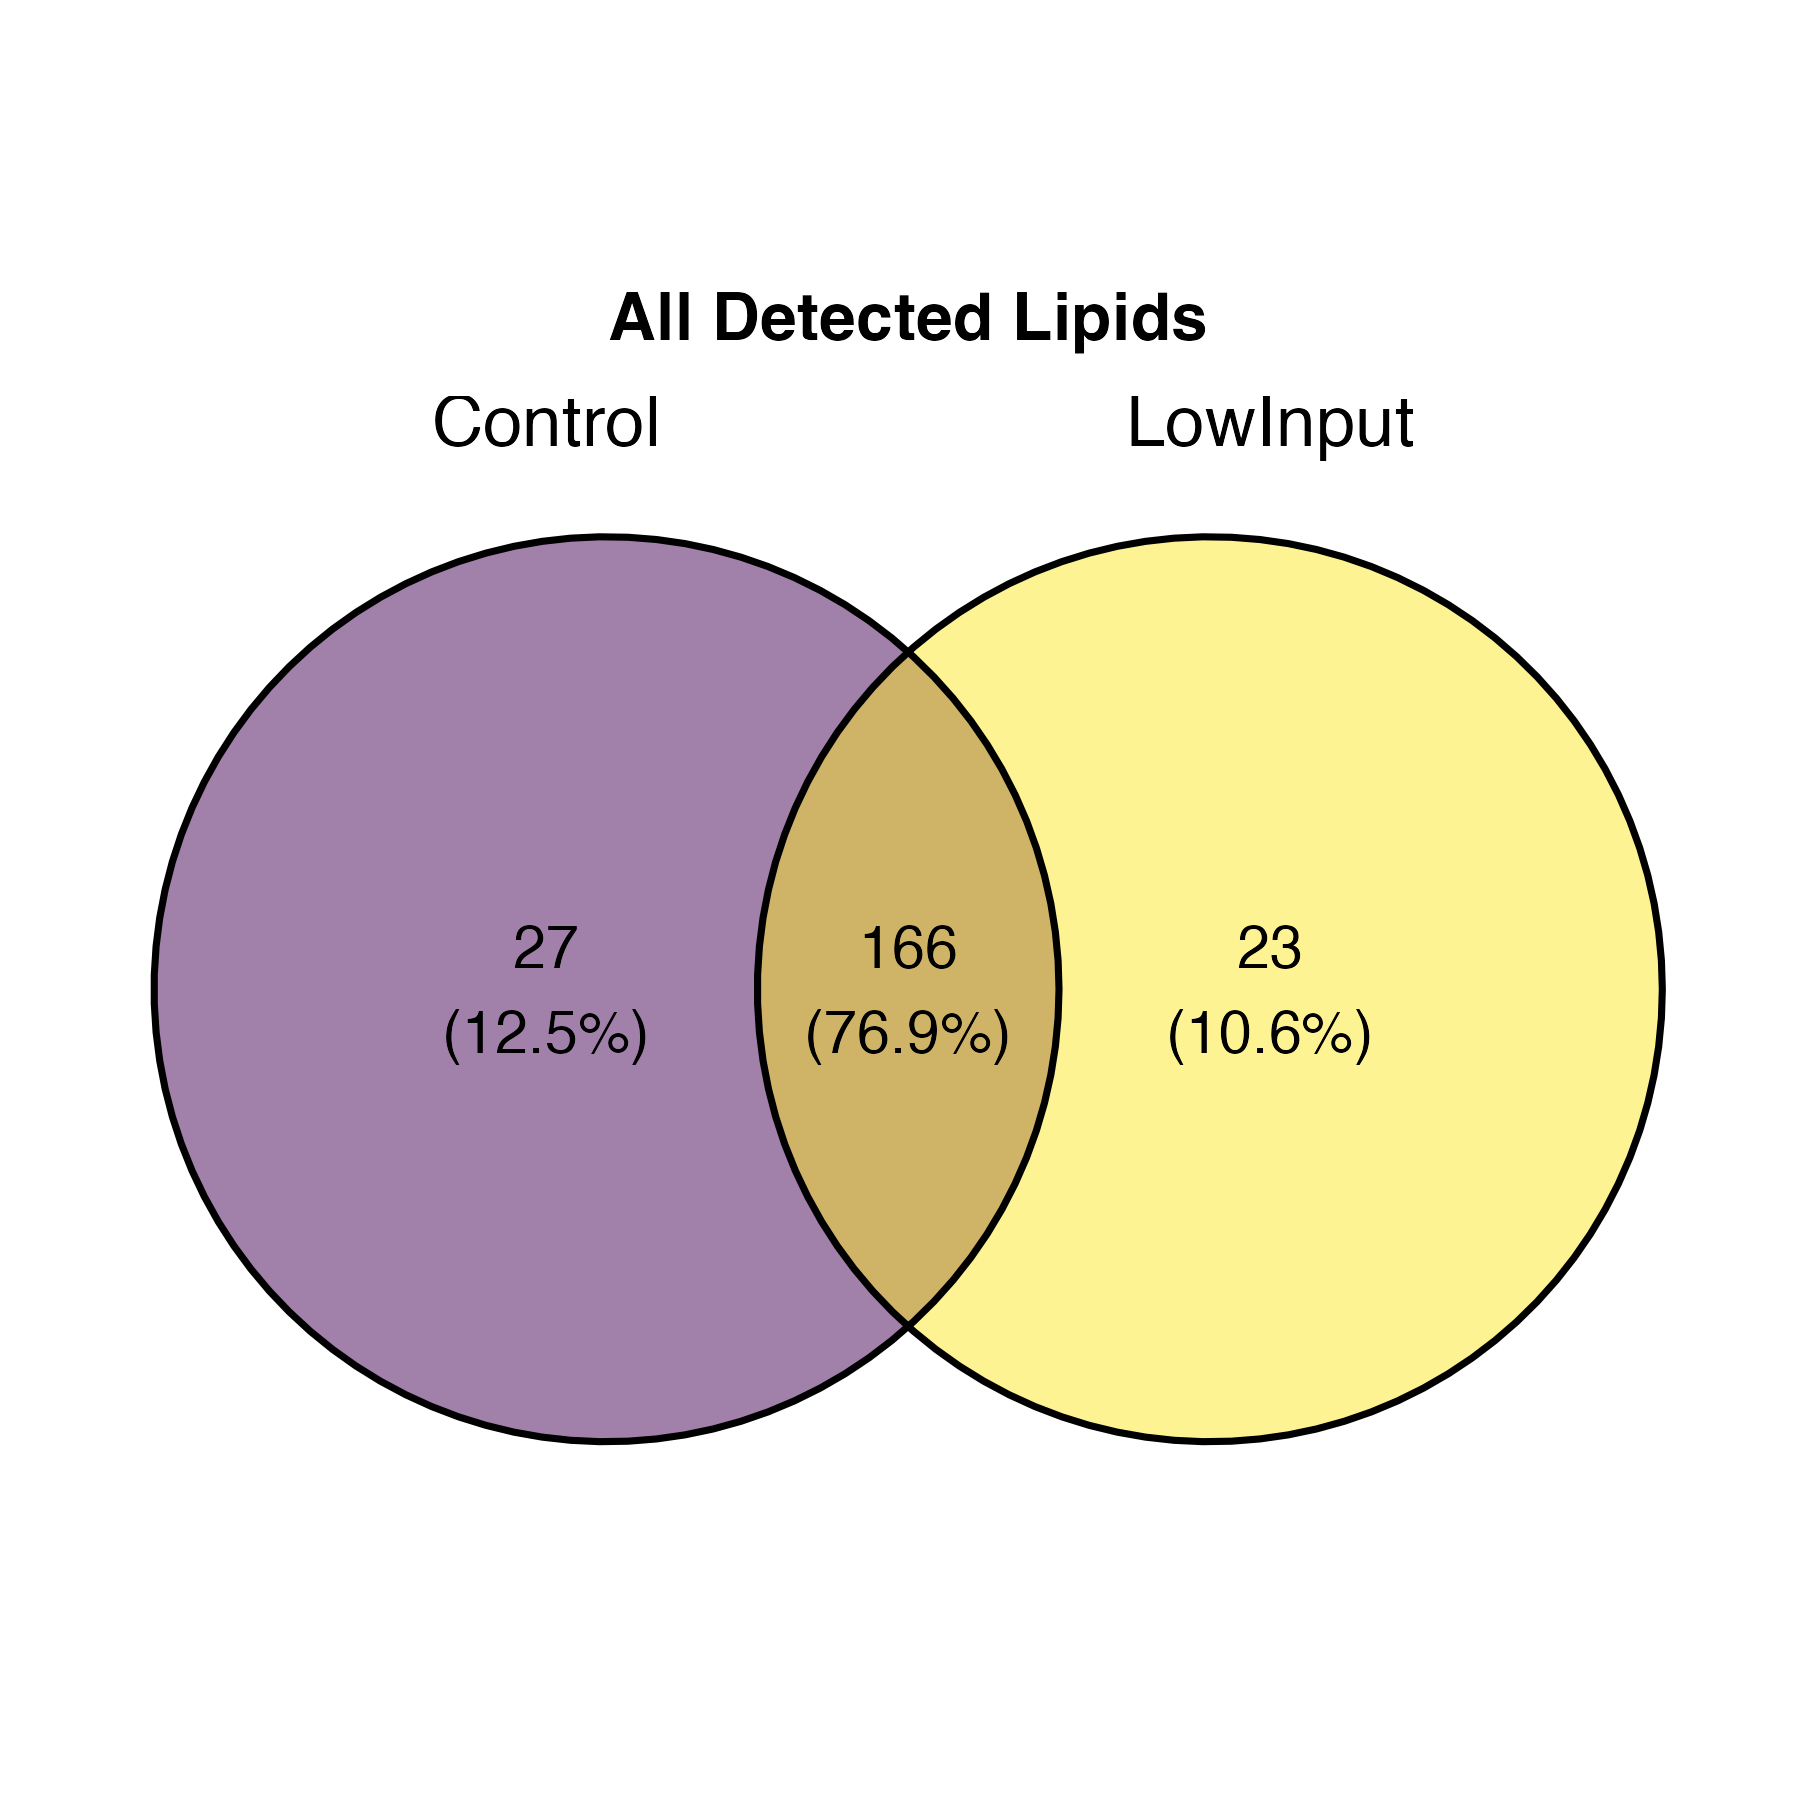
\includegraphics[width=\linewidth]{fig/supp/SuppFig_3C_Lipid_Overlap_Venn}
    \caption{Shared and unique lipid species.}
    \label{fig:S3C}
  \end{subfigure}

  \caption{Overview of lipid coverage in Control and Low-Input samples.}
  \label{fig:S3}
\end{figure}


%========================================================
%  Supplementary Figure S4 - Lipid ratio contrasts under low-P
%========================================================
\begin{figure}[htp]
  \centering
  % Adjust width fraction as needed (e.g., 0.8\textwidth or \textwidth)
  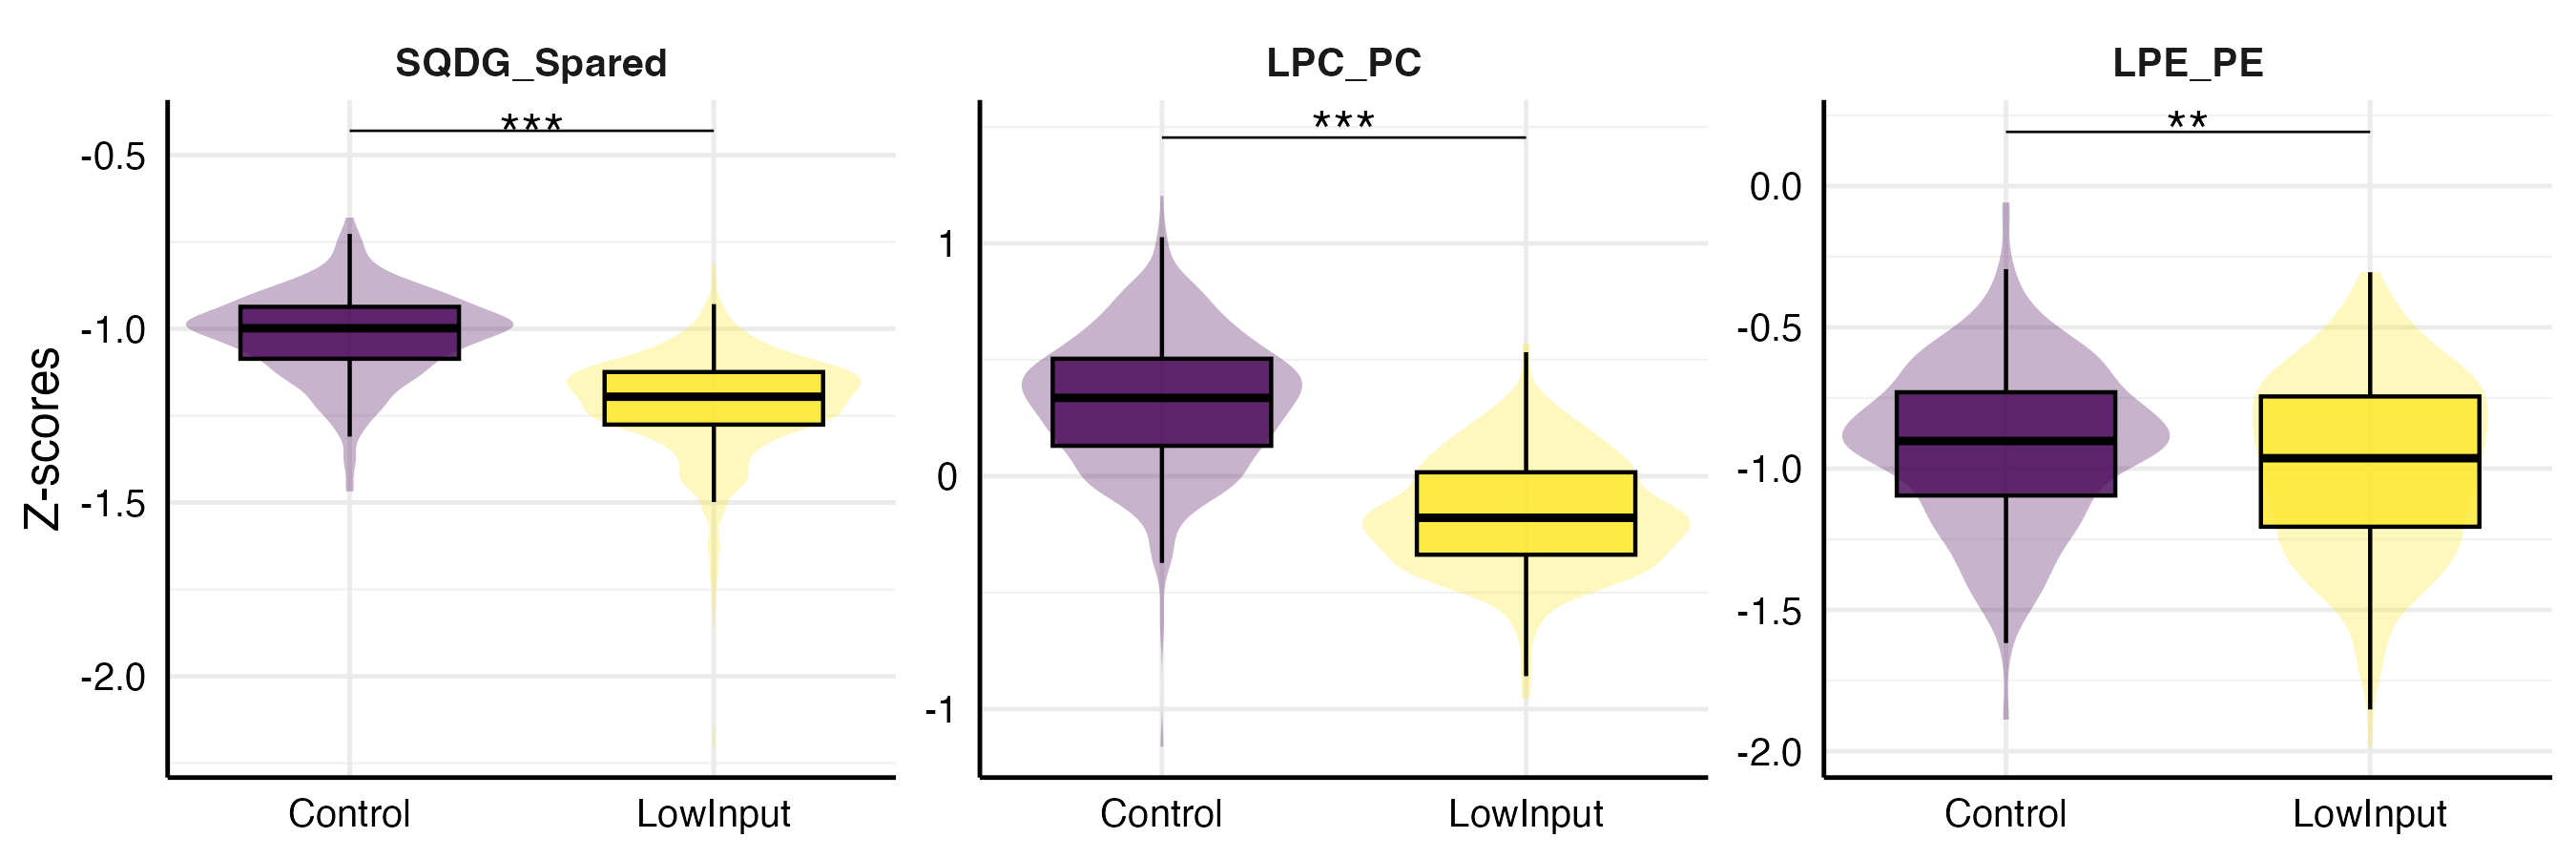
\includegraphics[width=0.8\textwidth]{fig/supp/SuppFig_4_lipid_ratio_linear_lowP.png}
  \caption{$\Delta$Z-score contrasts for lipids under LI. 
    The panel shows violin+boxplots for metrics such as \textitt{SQDG-Spared}, \textitt{LPC-PC}, and \textitt{LPE-PE} under Control versus LowInput conditions. 
    Stars denote significance levels (***: $p<0.001$, **: $p<0.01$, *: $p<0.05$) from appropriate statistical tests. 
    A negative $\Delta$Z in SQDG\_Spared indicates sulfolipid is not upregulated relative to galactolipids and PG; 
    \textitt{LPC-PC} is not significantly changed, whereas \textitt{LPE-PE} and composite Lyso\_activity shift toward values consistent with selective PE deacylation.}
  \label{fig:S4_lipid_ratio_lowP}
\end{figure}

%========================================================
%  Supplementary Figure S5 - TIC Proportions for LPC and LPE
%========================================================
\begin{figure}[htp]
  \centering
  % Adjust width fraction as appropriate, e.g., 0.6\textwidth or \textwidth
  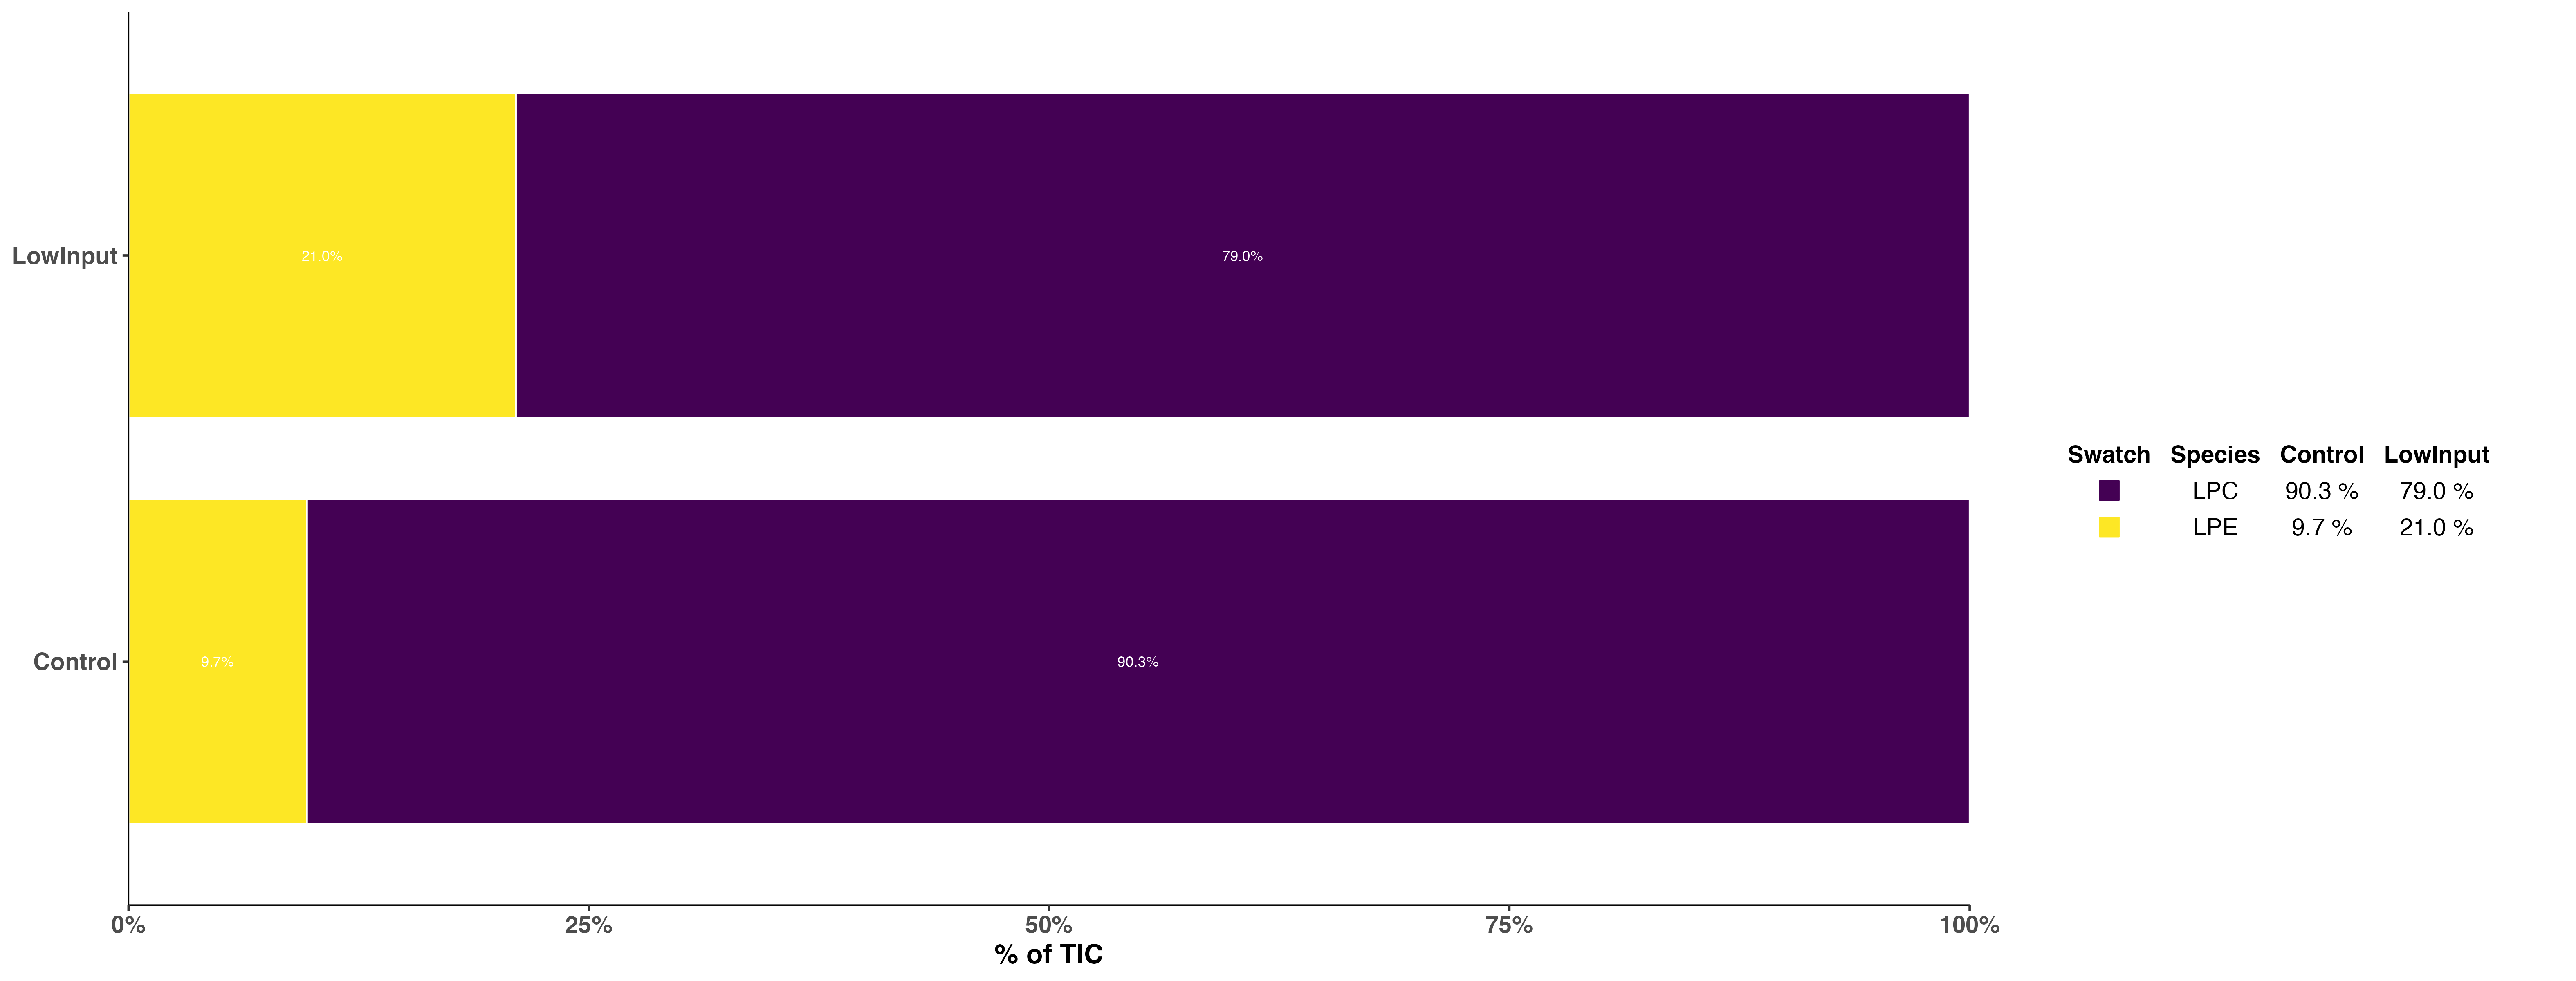
\includegraphics[width=0.7\textwidth]{fig/supp/SuppFig_5_TIC_LPC_LPE.png}
  \caption{Total ion current (TIC) proportions of lysophosphatidylcholine (LPC) and lysophosphatidylethanolamine (LPE) under Control and Low-P conditions. The plot displays relative TIC share of LPC versus LPE; stars denote significance levels (e.g., *: $p<0.05$, **: $p<0.01$) from appropriate tests. An increase in the LPE fraction and corresponding decrease in LPC under low-P suggests selective deacylation of PE for P salvage, while PC-derived LPC remains relatively stable.}
  \label{fig:S5_TIC_LPC_LPE}
\end{figure}



\end{document}


